%%%%%%%%%%%%%%%%%%%%%%%%%%%%%%%%%%%%%%%%%%%%%%%%%%%%%%%%%%%%%%%%%%%%%%
% Colorado State University LaTeX Thesis Template and Documentation
%
% by
%   Elliott Forney
%
% This is free and unencumbered software released into the public domain.
% 
% Anyone is free to copy, modify, publish, use, compile, sell, or
% distribute this software, either in source code form or as a compiled
% binary, for any purpose, commercial or non-commercial, and by any
% means.
% 
% In jurisdictions that recognize copyright laws, the author or authors
% of this software dedicate any and all copyright interest in the
% software to the public domain. We make this dedication for the benefit
% of the public at large and to the detriment of our heirs and
% successors. We intend this dedication to be an overt act of
% relinquishment in perpetuity of all present and future rights to this
% software under copyright law.
% 
% THE SOFTWARE IS PROVIDED "AS IS", WITHOUT WARRANTY OF ANY KIND,
% EXPRESS OR IMPLIED, INCLUDING BUT NOT LIMITED TO THE WARRANTIES OF
% MERCHANTABILITY, FITNESS FOR A PARTICULAR PURPOSE AND NONINFRINGEMENT.
% IN NO EVENT SHALL THE AUTHORS BE LIABLE FOR ANY CLAIM, DAMAGES OR
% OTHER LIABILITY, WHETHER IN AN ACTION OF CONTRACT, TORT OR OTHERWISE,
% ARISING FROM, OUT OF OR IN CONNECTION WITH THE SOFTWARE OR THE USE OR
% OTHER DEALINGS IN THE SOFTWARE.
%%%%%%%%%%%%%%%%%%%%%%%%%%%%%%%%%%%%%%%%%%%%%%%%%%%%%%%%%%%%%%%%%%%%%%

% Preamble
%%%%%%%%%%%%%%%%%%%%%%%%%%%%%%%%%%%%%%%%%%%%%%%%%%%%%%%%%%%%%%%%

% use the thesis document class
% this is derived from the standard book class
% and supports many of the same features
\documentclass[master]{thesis}
%\documentclass[doctor]{thesis} % for a dissertation

% fonts
% use times font by default but can specify other fonts
%\usepackage{fourier} % fourier is also a nice choice

%\usepackage[scaled]{helvet} % or these two lines give a sans-serif font
%\renewcommand\familydefault{\sfdefault} 

% this is useful for including dummy test
% it can be removed in final document
\usepackage{lipsum}

% ams math packages
\usepackage[cmex10]{amsmath}
\usepackage{amsthm,amssymb}

% graphics packages
\usepackage[pdftex]{graphicx} % remove pdftex if you are not compiling to pdf
\graphicspath{{./figures/}} % this places all graphics in the figures subdirectory

% allowed graphics extensions
% uncomment if you prefer to add extension in \includegraphics
\DeclareGraphicsExtensions{.pdf,.png,.jpg}

% allows the creation of subfigures
\usepackage[caption=false]{subfig}

% book tables are simple and look nice
\usepackage{booktabs}

% for specifying urls and links
\usepackage{url}
\urlstyle{same} % same style as regular text

% Title Page
%%%%%%%%%%%%%%%%%%%%%%%%%%%%%%%%%%%%%%%%%%%%%%%%%%%%%%%%%%%%%%%%

% title of your thesis
\title{Protein Interface Prediction Using Graph Convolutional Networks}

% author's name
\author{Alex M. Fout}

% author's email address
\email{fout@colostate.edu}

% department name
\department{Department of Computer Science}

% semester of completion
\semester{Fall 2017}

% committee member names
\advisor{Asa Ben-Hur}
\committee{Chuck Anderson} % as many committee entries as you need
\committee{Hamid Reza Chitsaz}
\committee{Wen Zhou}

% Copyright Page
%%%%%%%%%%%%%%%%%%%%%%%%%%%%%%%%%%%%%%%%%%%%%%%%%%%%%%%%%%%%%%%%

% here is an example of student copyright declaration
% note that the \copyright command prints the copyright symbol,
% so we use the name \mycopyright instead
\mycopyright{%
Copyright by Alex M. Fout 2017 \\
All Rights reserved
}

% here is an example of a creative commons copyright license
% ask the graduate school for more information
%\mycopyright{%
%This work is licensed under the Creative Commons Attribution-NonCommercial-NoDerivatives 3.0 United States License.
%
%\vspace{3em}
%
%To view a copy of this license, visit:
%
%\vspace{2em}
%
%\url{http://creativecommons.org/licenses/by-nc-nd/3.0/legalcode}
%
%\vspace{3em}
%
%Or send a letter to:
%
%\vspace{2em}
%
%Creative Commons
%
%171 Second Street, Suite 300
%
%San Francisco, California, 94105, USA.
%}

% Abstract
%%%%%%%%%%%%%%%%%%%%%%%%%%%%%%%%%%%%%%%%%%%%%%%%%%%%%%%%%%%%%%%%

\abstract{%
Abstract goes here.
}

% Acknowledgments 
%%%%%%%%%%%%%%%%%%%%%%%%%%%%%%%%%%%%%%%%%%%%%%%%%%%%%%%%%%%%%%%%

\acknowledgements{%
Acknowledgements go here.

Molecular graphics and analyses were performed with the UCSF Chimera package. Chimera is developed by the Resource for Biocomputing, Visualization, and Informatics at the University of California, San Francisco (supported by NIGMS P41-GM103311)
}

% Metadata
%%%%%%%%%%%%%%%%%%%%%%%%%%%%%%%%%%%%%%%%%%%%%%%%%%%%%%%%%%%%%%%%%%%%%%

% consider using hyperref to insert pdf metadata and make links clickable
% safe to remove if not using pdf or if it causes problems
\usepackage[pdfpagelabels,pdfusetitle,colorlinks=false,pdfborder={0 0 0}]{hyperref}

\begin{document} % preamble is complete, add any custom packages above
%%%%%%%%%%%%%%%%%%%%%%%%%%%%%%%%%%%%%%%%%%%%%%%%%%%%%%%%%%%%%%%%

\frontmatter % starts preliminary pages
%%%%%%%%%%%%%%%%%%%%%%%%%%%%%%%%%%%%%%%%%%%%%%%%%%%%%%%%%%%%%%%%

\maketitle
\makemycopyright
\makeabstract
\makeacknowledgements


\tableofcontents
\listoftables % optional
\listoffigures % optional

\mainmatter % starts thesis body
%%%%%%%%%%%%%%%%%%%%%%%%%%%%%%%%%%%%%%%%%%%%%%%%%%%%%%%%%%%%%%%%



%%%%%%%%%%%%%%%%%%%%%%%%%%%%%%%%%%%%%%%%%%%%%%%%%%%%%%%%%%%%%%%%

%TODO: refer to grid convolutions as discrete (?)


\chapter{Introduction}
\label{chap:intro}

Many cellular processes rely on proteins, which facilitate these processes via their interactions with one another and with small molecules within the cell~\cite{scheeffink2003}.
%TODO: mention protein interaction networks?
Understanding protein interactions is key to disease and pharmaceutical research, as well as our understanding of basic cellular biology~\cite{fauman2003, altman2003}.
Proteins normally interact via an \textit{interface}, a localized region of the protein with special properties.

Experimentally identifying the interface between two proteins is a time consuming and expensive process which involves crystallization of the protein complex and imaging via x-ray crystallography or nuclear magnetic resonance~\cite{bijelic2017, ilarisavino2017, wang2017}.
In contrast, computational methods are faster, cheaper, and complement wet lab experiments by identifying the most relevant and worthwhile experiments to attempt in vivo.

This thesis presents a novel computational method to predict the interface between a pair of interacting proteins.
The method is inspired by the success of convolutional neural networks in image processing~\cite{gu2015, lecun2010}, but adapts the ideas to this problem domain.
Proteins are represented as graphs and fed into a pairwise convolutional neural network with specialized convolution operations.
The network makes predictions on pairs of amino acid residues of the likelihood that they constitute a part of the interface. 
This method outperforms the existing state-of-the-art approach based on a support vector machine with pairwise kernels~\cite{minhas2014}.

%TODO: Update when done
The rest of this thesis is organized as follows.
The remainder of the introduction presents a primer on proteins and their interfaces. 
Chapter \ref{chap:relatedwork} reviews prior work in interface prediction.
Chapter \ref{chap:neuralnetworks} introduces neural networks and specifically convolutional neural networks.
Chapter \ref{chap:methods} describes the graph convolutional networks and the deep learning architecture used in this thesis.
Chapter \ref{chap:experiments} describes the data set and experiments performed and presents findings. 
Chapter \ref{chap:future} lays out potential avenues of research which build upon the findings in this thesis. 
Appendix \ref{appendix:features} contains details pertaining to the features computed for each amino acid residue, and Appendix \ref{appendix:tools} describes the software and tools that were created and/or used for this research.

\section{Proteins}

DNA is rightly considered the "blueprint for life," which begs the question, what is built from those blueprints?
The answer is, in many cases, the information contained in DNA is used to synthesize proteins.
Proteins are composed of amino acids linked in a chain and held together by covalent bonds.
Amino acids are organic compounds consisting of a central \textit{$\alpha$-carbon} atom, which binds to an \textit{amine group} ($\mathrm{NH_2}$), a \textit{carboxyl group} ($\mathrm{COOH}$), a single hydrogen atom, and a \textit{side chain}, in a tetrahedral geometry.
There are 21 unique amino acids encoded in eukaryotic DNA, each of which has a distinct side chain that gives rise to structural and electro-chemical properties.
Figure \ref{fig:aminoacids} depicts the different amino acids.

\begin{figure}
	\centering
	%\begin{center}
	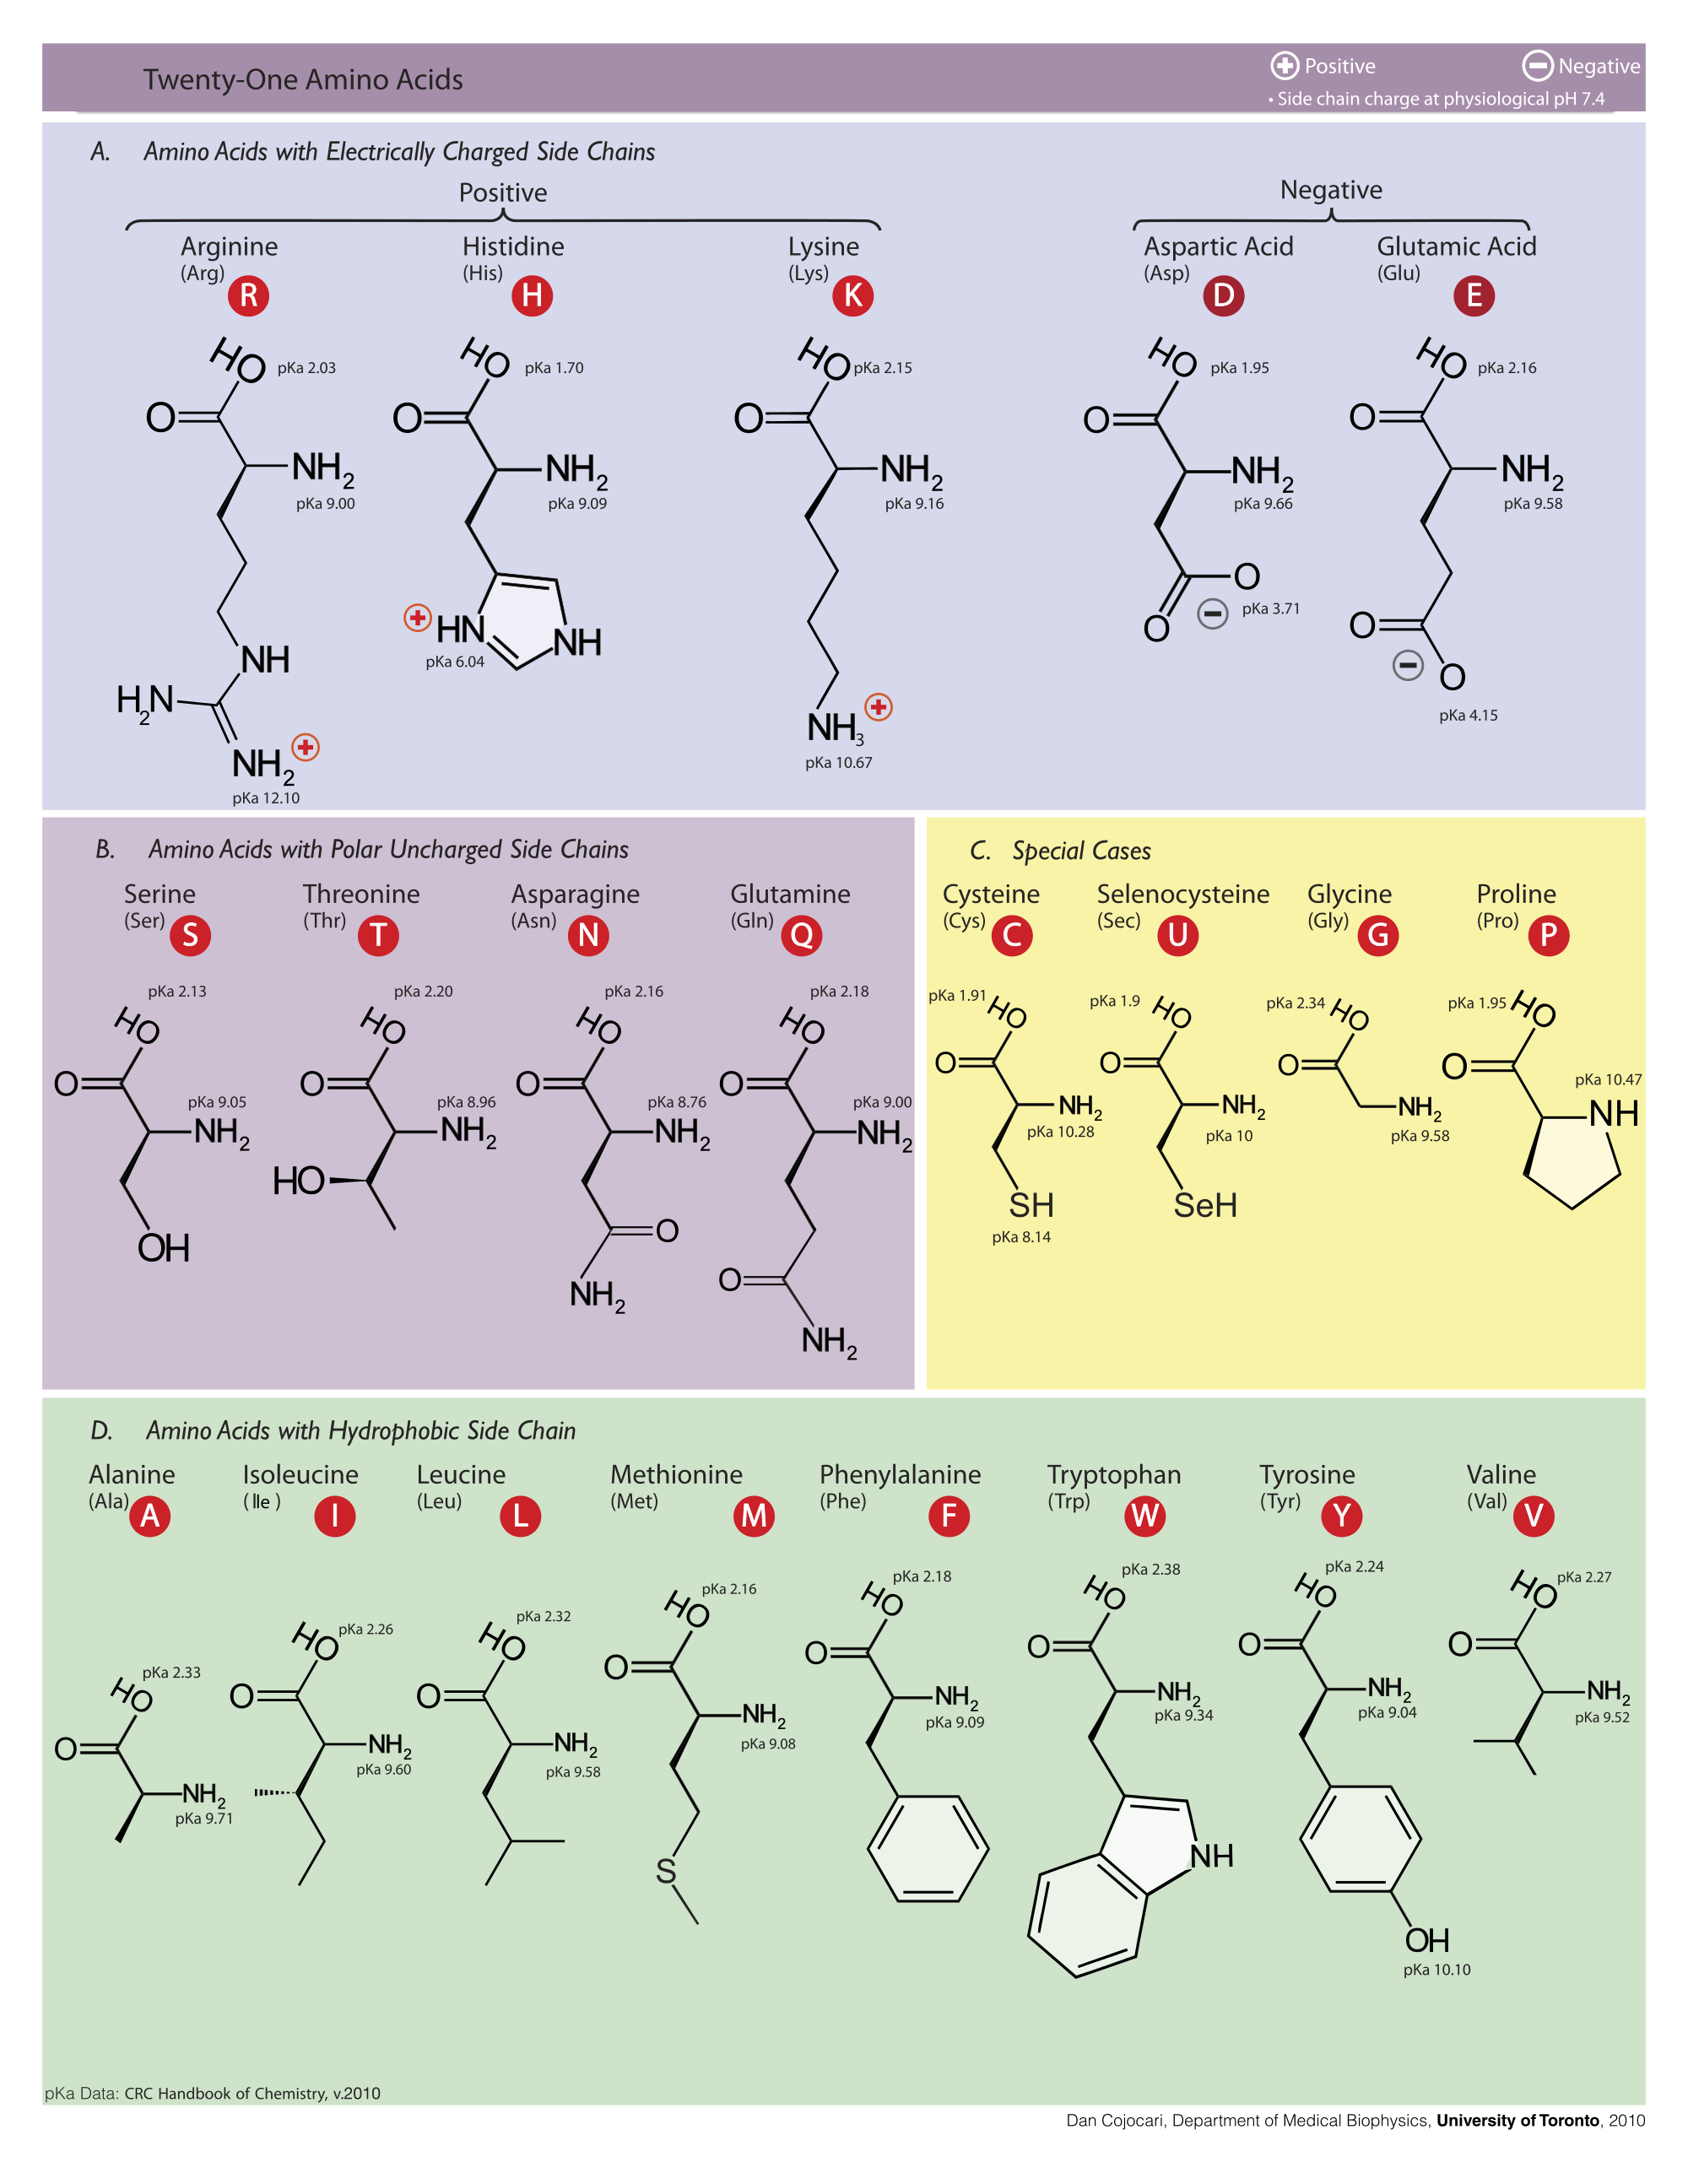
\includegraphics[width=0.8\textwidth]{Molecular_structures_of_the_21_proteinogenic_amino_acids.png}
	%\end{center}
	\caption{The 21 types of amino acid encoded in eukaryotic DNA, chategorized by their electrical properties. Full names, along with three letter and single letter abbreviations are given. Chemical structures are oriented so that the carboxyl group, $\alpha$-carbon, and amine groups are on top, with the side chain extending downwards.}
	\label{fig:aminoacids}
\end{figure}
%TODO: How to include liscence for this figure?

Two amino acids link together when the nitrogen atom from one's amine group bonds covalently with the carbon atom of another's carboxyl group, releasing a water molecule in the process.
This covalent bond is called a peptide bond, and an amino acid involved in at least one such bond is referred to as an \textit{amino acid residue}, or \textit{residue}.

A \textit{peptide}, or \textit{peptide chain}, is a linear chain of amino acids held together by peptide bonds, and the \textit{backbone} of the peptide consists of all atoms participating in peptide bonds, together with the $\alpha$-carbons.
If a peptide contains several residues it is referred to as a \textit{polypeptide}.
Proteins consist of one or more polypeptides which are bound together.
All peptides have a canonical ordering, from the \textit{N-terminus}, the residue with a free amine group, to the \textit{C-terminus}, the residue with a free carboxyl group.
This matches the order that polypeptides are created during biological protein synthesis.
Figure \ref{fig:3res} shows a ball and stick model of a small peptide.

\begin{figure}
	\centering
	%\begin{center}
	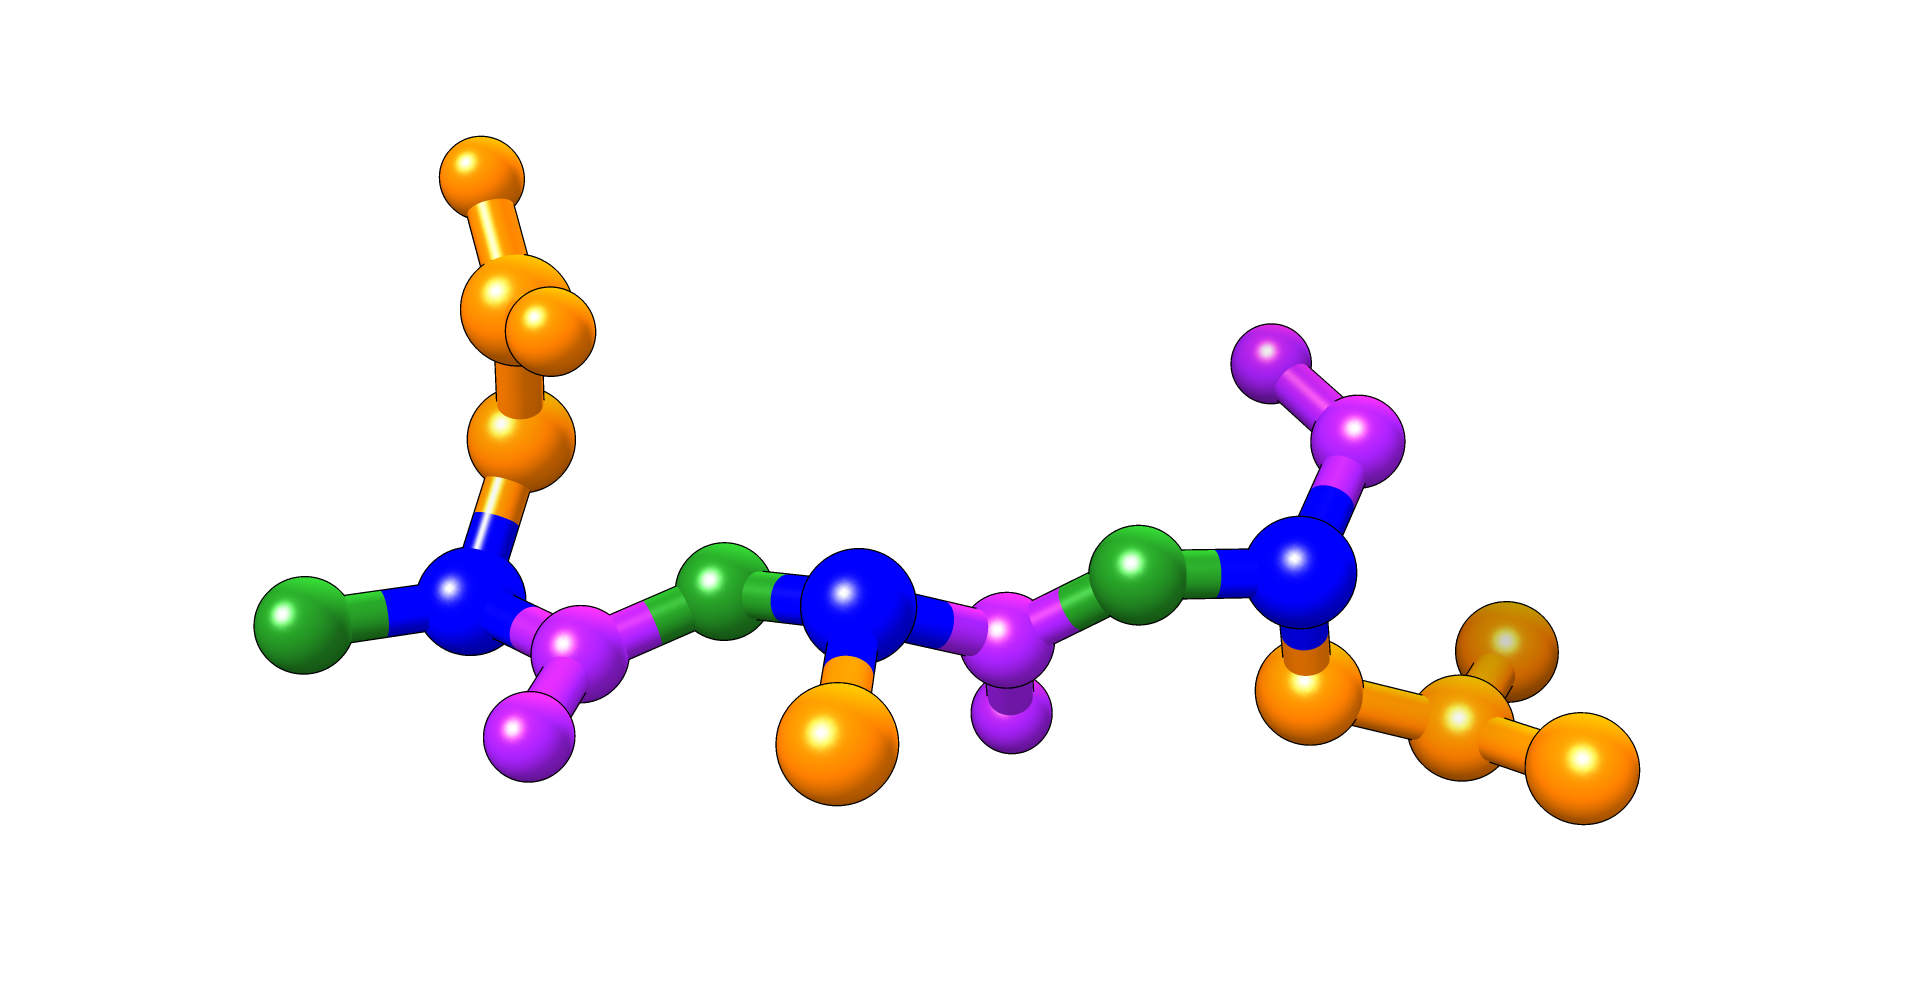
\includegraphics[width=0.8\textwidth]{1dab_3res_3x3.png}
	%\end{center}
	\caption{Ball and stick model of a peptide containing three amino acid residues (hydogens omitted). Colors indicate, blue: $\alpha$-carbon , orange: side chain, purple: carboxyl group after loss of OH, green: amine group after loss of H. Peptide bonds are between purple and green atoms. The backbone extends horizontally along blue, purple, and green atoms. Each sequence of atoms starting at an $\alpha$-carbon and ending at the next $\alpha$-carbon lay in an amide plane. From left to right are Aspartic Acid, Alanine, and Leucine. Created with Chimera~\cite{pettersen2004}.}
	\label{fig:3res}
\end{figure}

A residue's side chain influences how it interacts with other amino acids or other atoms and molecules. 
For example, oppositely charged side chains are be attracted to each other.
Polar side chains, being hydrophilic, are attracted to water molecules, and non-polar side chains, being hydrophobic, will prefer to avoid water and other polar molecules.
Such interactions play an important role in how proteins fold into 3D structures \cite{scheeffink2003}.

%TODO: mention globular proteins vs other kinds?


\subsection{Protein Structure}

Protein structure can be described via four levels of abstraction, termed \textit{primary}, \textit{secondary}, \textit{tertiary}, and \textit{quaternary} structure.
Primary structure refers to the sequence of amino acid residues (from N-terminus to C-terminus) in a single polypeptide, and is determined by the sequence of codons in the corresponding coding mRNA from which the protein is translated.
Sequences are typically written using a string of letters, where each unique letter corresponds to a different residue type. 

The physical chemistry associated with peptide bonds gives rise to the property that the nitrogen and carbon atoms involved in the peptide bond, along with the adjacent $\alpha$-carbons, all lie within a plane, called the \textit{amide plane}.
Each $\alpha$-carbon lies on the intersection between two amide planes, and the planes are free to rotate with respect to each other. 
%TODO: figure?
In some cases, side chains prohibit certain relative angles due to \textit{steric constraints}, which enforce that no two atoms may occupy the same volume of space at the same time.
In general, however, the angle between amide planes provides flexibility in the peptide backbone, which allows for the formation of higher order structures.

Secondary structure describes the local 3D structures that arise from the attraction of non-adjacent residues in a polypeptide.
There are three common categories of local structures: $\alpha$-helices, $\beta$-sheets, and loops.
An  $\alpha$-helix occurs when the polypeptide coils into a barrel-like structure (like the threads of a screw) and residues from adjacent coils (a distance of three residues from each other along the backbone) form hydrogen bonds with one another.
A $\beta$-sheet occurs when two non-adjacent sections of the polypeptide align next to each other such that residues in one of the sections form hydrogen bonds with residues in the other section.
$\beta$-sheets may be parallel or anti-parallel, depending on the relative orientation of adjacent strands in the sheet.
Figure \ref{fig:beta} illustrates the difference between parallel and anti-parallel $\beta$-sheets.
\begin{figure}
	\centering
	%\begin{center}
	\subfloat[Parallel $\beta$-sheets]{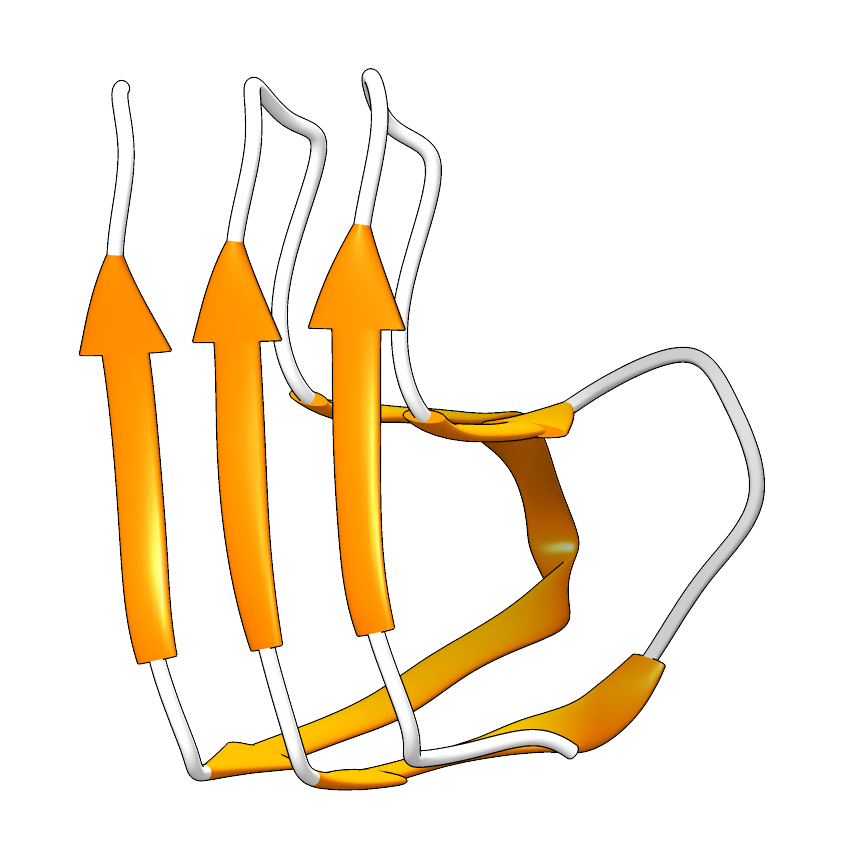
\includegraphics[width=0.4\textwidth]{1dab_end_betaP_3x3_cropped.png}\label{fig:beta_para}}
	\hfill
	\subfloat[Anti-parallel $\beta$-sheets]{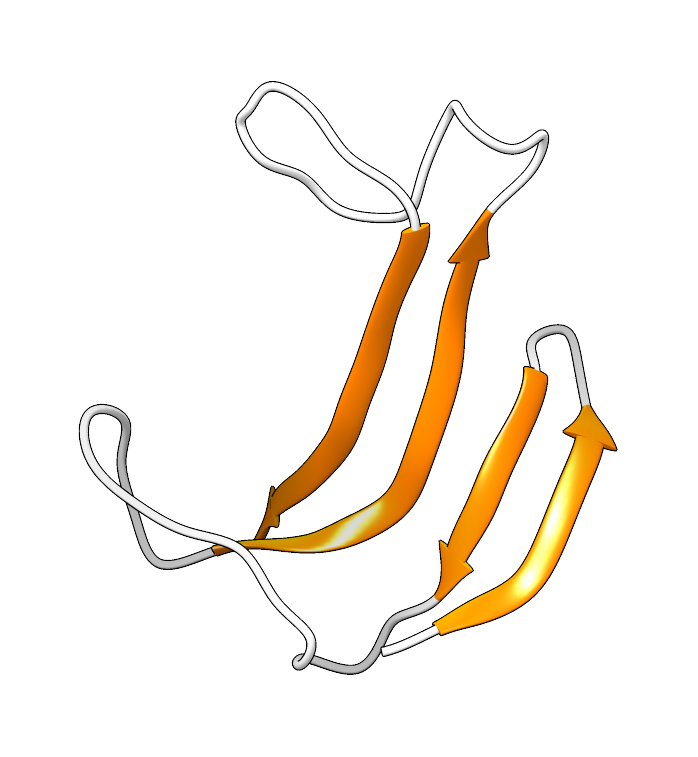
\includegraphics[width=0.4\textwidth]{1ca2_part_betaA_3x3_cropped.png}\label{fig:beta_anti}}
	%\end{center}
	\caption{Cartoon examples of parallel and anti-parallel $\beta$-sheets. In parallel $\beta$-sheets, adjacent strands in the sheet are oriented the same way, whereas in anti-parallel $\beta$-sheets, adjacent strands are oriented opposite each other. Created with Chimera~\cite{pettersen2004}.}
	\label{fig:beta}
\end{figure}
Some sections of the polypeptide form neither helices nor sheets, and are called loops.
These sections are more flexible than helices or sheets due the lack of hydrogen bonds, and therefore are useful in connecting the end of one helix/sheet to the beginning of another.
Figure \ref{fig:5nji_ss} shows a cartoon depiction of part of a protein, with different secondary structural elements highlighted in different colors.
	
\begin{figure}
	\centering
	%\begin{center}
	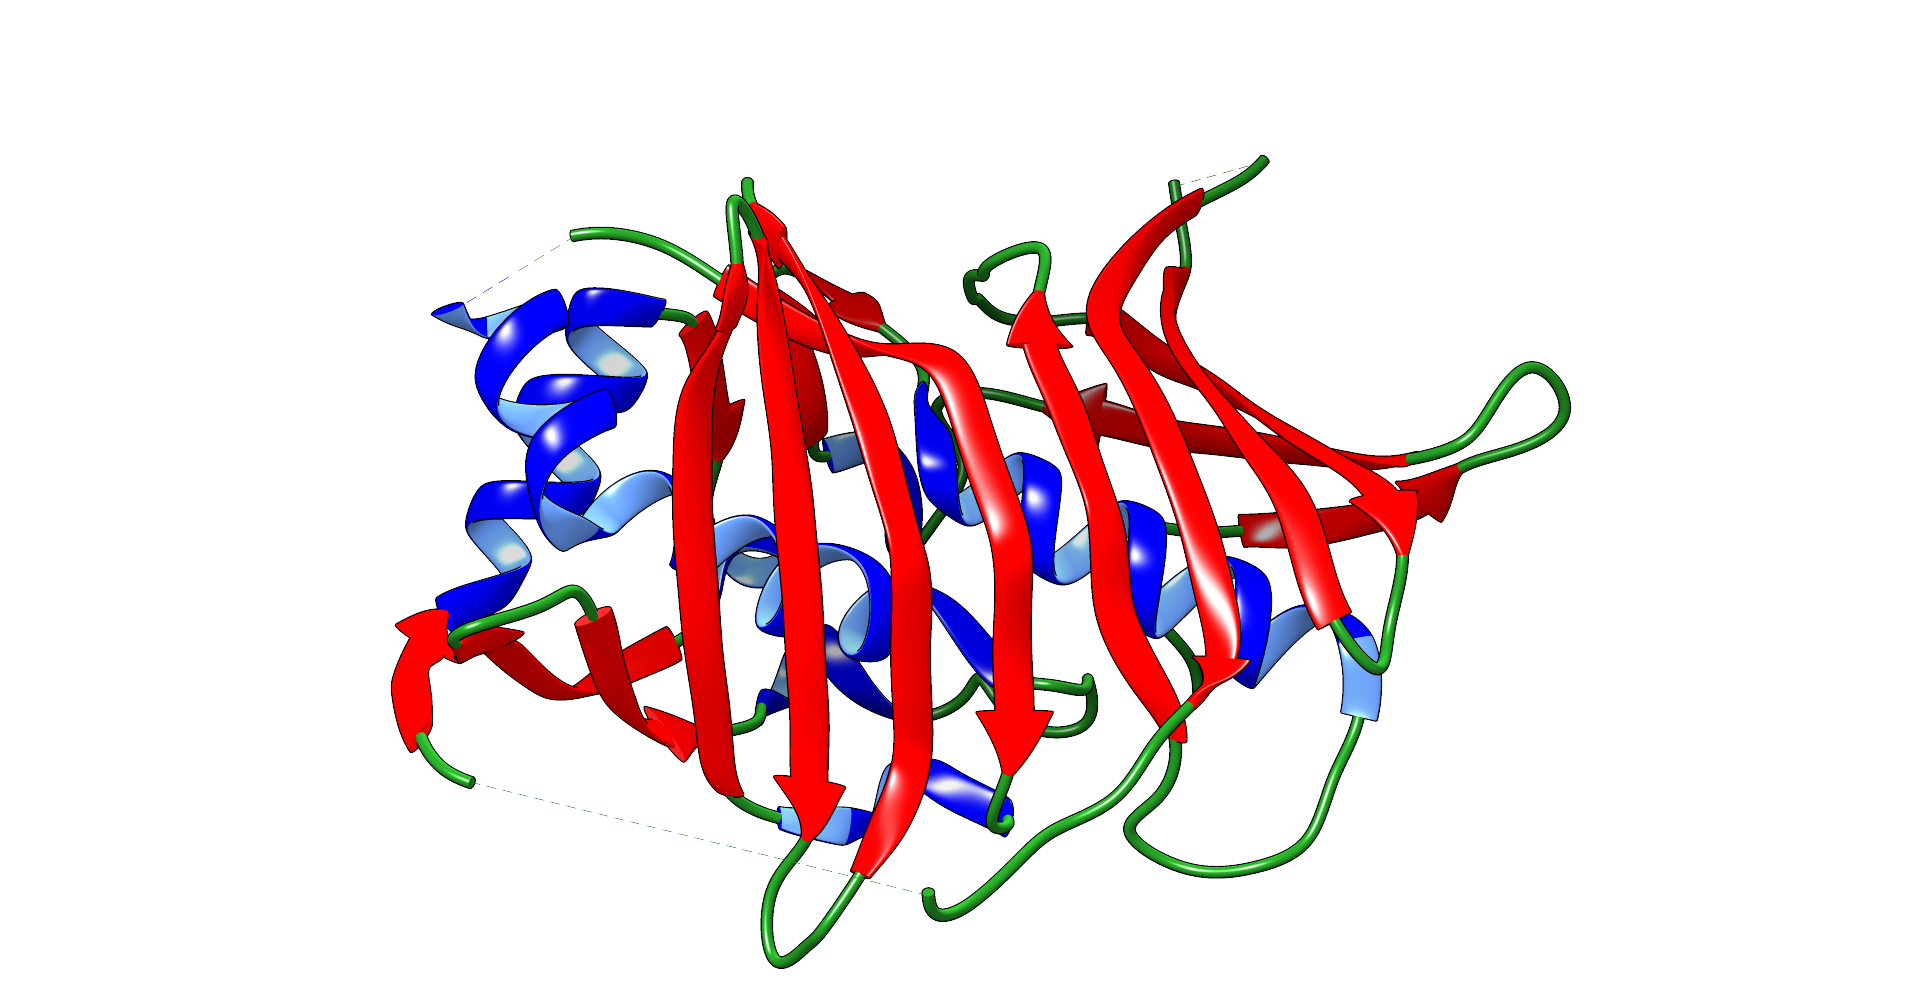
\includegraphics[width=0.8\textwidth]{5nji_ss_ch_3x3.png}
	%\end{center}
	\caption{3D cartoon of the the dehydratase domain of PpsC protein from Mycobacterium tuberculosis (PDB entry 5NJI~\cite{faille2017}) showing $\alpha$-helices in blue, $\beta$-sheets in red, and loops in green. Created with Chimera~\cite{pettersen2004}.}
	\label{fig:5nji_ss}
\end{figure}

Helices and sheets provide some rigidity to a polypeptide, but it typically further folds into a larger, tertiary structure, which may be globular, fibrous, or such that they reside on a cellular membrane.
After folding, some residues reside on the surface while others are buried in the core.
Because water makes up the majority of the cellular environment, protein surfaces have a higher percentage of hydrophilic residues than cores, and cores likewise have a higher percentage of hydrophobic residues than surfaces. 
Protein cores also show higher evolutionary conservation compared to surfaces~\cite{yan2008}.


Finally, in many cases multiple polypeptides combine together into a complex~\cite{scheeffink2003}.
%complexes may be \textit{obligate}, meaning they persist 
Quaternary structure describes the manner in which the individual polypeptides, known as subunits in this context, combine together to form the complex.
Protein complexes can be categorized as either \textit{transient} or \textit{permanent}.
This distinction reflects the difference in binding affinity (strength of attraction) between single proteins in the complex, with permanent complexes having higher and transient complexes having lower affinity.
Complexes can also be categorized as either \textit{obligate} and \textit{non-obligate}.
The constituent proteins of obligate complexes typically exist only in the complex, whereas for a non-obligate complex, each constituent protein exists both in the complex and independently.
Transience usually implies non-obligation and obligation usually implies permanence, so a simpler classification of obligate vs. transient is also appropriate~\cite{jones1996, perkins2010}.
The temporary nature of transient interactions enables complex networks of interaction which give rise to numerous cellular processes and the regulation thereof~\cite{perkins2010, ofran2003}.
Proteins in which all subunits are identical are called homomeric whereas proteins with different subunits are called heteromeric.
Homomeric proteins are usually obligate and more conserved than heteromeric proteins~\cite{jones1996}\cite{yan2008}

% receptor-ligand interaction and signal transduction.
% example of each: substrate-level phosphorylation, protein hormones, transcription factors, antibodies.


\subsection{Protein Interfaces And Their Prediction}

%TODO: mention ligand and receptor

The locus of a protein-protein interaction is the interface, which is comprised of pairs of residues, one from each interacting protein.
These pairs may form a disulfide bond or salt bridge which help anchor the two proteins together~\cite{yan2008}, but this is not always the case~\cite{ofran2003}.
Residues may not attract each other directly but still be considered part of the interface due to their proximity.
This is the case when hydrophobic residues from two proteins appear near each other in the interface, since they do not attract each other, but this configuration is energetically favorable compared to being exposed to water in the surrounding cytoplasm~\cite{yan2008, ofran2003}.
Historically, residues have been considered part of the interface if they are in contact with residues on the adjacent protein. 
This is typically determined in one of two ways, either the distance between any atom in the residue in question and any atom in the other protein is below a threshold, or the exposed area of a residue drops sufficiently after complex formation. ~\cite{yan2008, jones1996, ofran2003, minhas2014}.

A survey of known protein complex structures from the Research Collaboratory for Structural Bioinformatics (RCSB) Protein Data Bank (PDB)~\cite{berman2000} has shown that interfaces have a higher prevalence of hydrophobic residues, lower prevalence of hydrophilic residues, and more evolutionary conservation compared to non-interface surface regions~\cite{yan2008}.
The higher overall hydrophobicity of an interface region biases the protein towards configurations in which the interface excludes water by binding to another protein.
The higher degree of conservation shows the functional significance of the interfaces, although conservation is somewhat lower for transient compared to obligate complexes~\cite{jones1996}.
Transient complexes also have a comparatively~\textit{lower} hydrophobicity compared obligate complexes, consistent with the fact that proteins in transient complexes exist outside of the complex, with interfaces exposed to water~\cite{jones1996}.
To overcome the unfavorable energetic effects of burying more hydrophilic residues in an interface, transient interfaces also have relatively higher numbers of hydrogen bonds~\cite{jones1996}.
It has also been shown that transient complexes have less shape complementarity between the participating proteins compared to obligate complexes~\cite{jones1996}.
Lastly, transient interfaces also tend to either be smaller in size (for weakly interacting complexes)~\cite{jones1996, perkins2010}, or undergo more conformational change when forming (for strongly interacting complexes)~\cite{perkins2010} compared to obligate complexes.
These differences make transient complexes more difficult to distinguish from non-interface surface residues~\cite{perkins2010}.

Historically, the problem of interface prediction has been formulated in two ways: \textit{partner-independent} and \textit{partner-specific} prediction.
The former variant considers a single residue from a protein and attempts to answer the question: does this residue form part of the interface with some other partner protein?
The latter variant considers pairs of residues, each from a different protein, and attempts to answer a more specific question: does this \textit{pair} of residues constitute part of the interface between these two proteins?
The pairwise nature of partner-specific prediction allows the consideration of the compatibility of a pair of residues, which has been found to increase performance~\cite{ahmad2011, minhas2014}.
Methods of interface prediction include \textit{docking methods}, \textit{template-based methods}, and \textit{machine learning methods}.

Docking methods predict the 3D bound formation of two proteins in a complex, from which the interface can be extracted. 
These methods use energy minimization techniques~\cite{chen2003, zundert2016}.
Unlike template and machine learning methods, docking methods do not require a library of known interfaces in order to make predictions, but are historically poor at accounting for conformational change during complex formation~\cite{ezkurdia2009}.

Template based methods make predictions based on similar known interfaces.
The protein of interest is compared to a library of interfaces, and the interface is predicted from the most similar interfaces from the library.
Template methods rely on a non-redundant library and can make predictions only when there is a sufficiently close match to an interface in the library~\cite{tuncbag2011}.

Machine learning methods attempt to directly predict the interface rather than comparing against a template complex or predicting the bound formation, however they still use information from a library of complexes whose interfaces are known.
Machine learning approaches have included use of neural networks and support vector machine~\cite{ahmad2011}~\cite{minhas2014}.
The latest SVM based approach, PArtner-specific Interacting Residue PREDictor (PAIRpred), uses pairwise kernels which operate on pairs of residues and incorporates both sequence and structural information of residues.
The method performs well compared to existing docking and machine learning methods~\cite{minhas2014}. More detail of prior work in interface prediction will be given in Chapter \ref{chap:relatedwork}.



\chapter{Prior Work In Interface Prediction}
\label{chap:relatedwork} 

%In silico prediction of interfaces began in the 

As previously mentioned, the experimental determination of protein complexes is time and resource intensive, prompting computational modeling approaches.
Esmaielbeiki et al describe three slightly different objectives in this vein, protein interaction prediction, protein-protein docking, and protein interfaces prediction~\cite{esmaielbeiki2015}.
The first objective seeks to identify pairs of proteins which interact, elucidating the complex protein interaction networks that give rise to cellular processes. 
The second objective considers two specified proteins and seeks the bound 3D structure of their complex.
The third objective, and the focus of this thesis, is chiefly concerned with identifying the specific residues or pairs of residues which make up the interface between two proteins.
It is less concerned with the 3D complex structure as with the interface itself.

It is worth noting that docking methods can also be used to predict interfaces, by first solving for the 3D structure of the complex and then extracting the interface from the complex.
Indeed, docking methods were some of the earliest computational approaches developed to model protein interactions~\cite{janin1995}.
Docking begins with the known unbound structures of two proteins known to interact, and conducts two main steps: search and scoring.
During search, two proteins are translated and rotated relative to each other and brought into contact to create a putative 3D bound structure for the complex.
The putative structures are then evaluated by a scoring function to identify the structures that are most likely to be part of the complex.
Docking methods differ in their the search algorithm and scoring function.
Scoring functions may incorporate complementarity in geometry, chemistry, and electrostatics, or incorporate van der Walls forces or evidence based (aka statistical) potentials~\cite{tuncbag2011}\cite{janin1995}.
One of the major advantages of docking is its ability to produce interface predictions \textit{ab initio} without requiring examples of known interfaces, which is particularly useful when experimental complex data are sparse.
Unfortunately, docking methods traditionally suffer from relatively high false positive rates, are considerably less effective for complexes which undergo conformational change when binding, and are computationally expensive because of the vast search space~\cite{janin1995}\cite{tuncbag2011}.

Some early alternatives to docking also avoided using example 3D bound structures, instead relying on sequence information, residue properties, and unbound structures for each protein in the complex.
Lichtarge et al~\cite{lichtarge1996} used inferred evolutionary relationships between different proteins to identify conserved residues and then identified those conserved residues which lay on the surface of the protein.
This method was based on the hypothesis that conserved surface residues must be vital to a protein's function and therefore probably constitute an interface.
Pazos et al~\cite{pazos1997} take a similar approach, but instead look at evolutionary relationships between protein complexes and identify pairs of residues between the proteins in the complex which have co-evolved.
This method requires only sequence information and therefore is applicable even in cases where the protein structures are unknown. 
Additionally, this method is partner specific since it identifies residue pairs which show correlated changes.
Gallet et al~\cite{gallet2000} use a sliding window on a protein sequence and calculate measures of hydrophobicity in a region, which can easily be calculated knowing the residue identities and secondary structure.
This method requires no phylogenetic information so is applicable even when no close evolutionary relatives can be identified.

Early methods such as those listed above were crafted for the available data and computational resources of the time, but were unable to fully account for the growing body of research surrounding protein interfaces and their properties as in (Jones \& Thornton, 1996)~\cite{jones1996}.
It was (Jones \& Thornton, 1997) that proposed a method which incorporated multiple structural features such as surface planarity, planarity, and accessible surface area, with residue level features such as solvation potential, hydrophobicity, and interface residue propensity.
They constructed a manual scoring function which inputs were the aforementioned features and output was a score, where higher scores corresponded with members of the interface.
They constructed a different scoring function for each of three different categories of complex, reflecting observations made into the characteristics of different complex types.
Prediction was performed on patches of residues.

Evaluation of early methods was challenging due to the paucity of experimentally determined protein interfaces~\cite{esmaielbeiki2015}.
Thankfully, the turn of the twenty first century coincided with an increase in the number of experimentally determined structures added to only databases such as the Protein Data Bank~\cite{berman2000}
Curated subsets also emerged which focused on evaluating protein-protein docking methods, such as the Critical Assessment of Predicted Interactions (CAPRI)~\cite{janin2003} and the Docking Benchmark Dataset (DBD)~\cite{chen2002}.
These subsets also became useful in the evaluation (and sometimes training) of interface detection methods.
	
This increasing availability of data and increased interest in the problem led to a growing number and diversity of approaches.
The emergent of class known as \textit{template based} methods utilized a non-redundant library of known protein interfaces to make predictions about unforeseen proteins.
For a given query protein, a search is made in the library for known complexes where one partner is similar to the query protein.
The interface of the query protein is then inferred from the interfaces of the most similar query results.
Similarity may be measured via homology (sequence similarity) or structural similarity~\cite{esmaielbeiki2015}.


Increased data and interest led to growing number and diversity of approaches.
	larger libraries allow matching of structure to a template (homologous/sequence or structure)
	
	growth of statistical and machine learning approaches
		svm
		nn
		naive bayesian
		hmm
		conditional random field
	typically incorporate both sequence and structure information and information from sequential/structural neighbors
	not global solutions like docking
	still partner independent
	
zhou and qin identify need for partner specific methods to increase specificity of predictions (zhou 2007)
		



\section{Pairwise Methods}




Interfaces exhibit a local spatial correlation in that a residue is more likely to be a part of an interface if nearby residues are also a part of the interface. 
Local spatial correlation can aid prediction if information from nearby residues is taken into account during prediction.


Such methods exist, but are often based on energy minimization techniques which are computationally expensive and attempt to model the entire 3D structure of the interface at once~\cite{esmaielbeiki2015}.
Some of these methods (Haddock~\cite{zundert2016} for example) allow the user to suggest amino acid residues which are likely part of the interface, to help bias the algorithm towards a correct solution.
This has motivated work to predict amino acid pairs which constitute part of the interface without solving for the entire interface at once. 






%\chapter{Artificial Neural Networks}
\label{chap:neuralnetworks}

\textit{Feed forward artificial neural networks}, or less formally, \textit{neural networks}, are a class of machine learning algorithms which are loosely inspired by neuroscientific models of how biological neural networks operate\cite{mcculloch1943}. 
Like many machine learning methods, a neural network is a parameterized function with vector input and either scalar or vector output.
For example, the input may be pixel intensities from an image of interest, and the output may be an integer corresponding to a label which indicates the image's content.
In this thesis, the function is denoted $f(x|\Theta)$, where $x$ is the input vector and $\Theta$ is the complete set of parameters, or weights.
In neural networks, $f$ is composed of a sequence of layers, $h_i(x_i|\Theta_i)$, which perform comparatively simple mathematical operations on their input to produce a layer output.
By convention, the input vector is considered the first layer of a neural network, even though it performs no operations, and the output of the last layer is the output of the entire network.
All intermediate layers are termed \textit{hidden layers}, each of which accepts the output of the preceding layer and passes its output to the subsequent layer.
The number of layers in a neural network (besides the first layer) is its \textit{depth}, and the number of outputs of a given layer is the number of \textit{units} (or \textit{neurons}) in that layer.

A common form of hidden layer is a \textit{dense layer}, in which each unit calculates a weighted sum of the layer inputs, where the set of weights is unique to each unit.
It is also common to add a scalar bias term and apply a nonlinear activation function to the weighted sum.
Dense layers have a convenient mathematical representation:

\begin{equation}
h(x|W, b)=\sigma(W x^T + b),
\label{eq:denselayer}
\end{equation}

\noindent
where $W$ is a matrix of weights, $x$ is the layer input, $b$ is a vector of biases, and $\sigma(\cdot)$ is a nonlinear activation function.
If there are $n$ inputs to a layer and $m$ units in the layer, then $W\in\mathbb{R}^{nxm}$ and $b\in\mathbb{R}^{m}$.
The expression $W x^T + b$ is the \textit{signal}, and $h$ is the \textit{activation}.
For hidden layers, activations have traditionally taken the form of a sigmoidal, or "s-shaped", function such as the logistic function, $\sigma(x) = 1/(1+e^{-x})$, or hyperbolic tangent, $\sigma(x) = tanh(x)$.
Figure \ref{fig:twolayernetwork} shows a graphical depiction of a simple two layer neural network.

\begin{figure}
	\centering
	%\begin{center}
	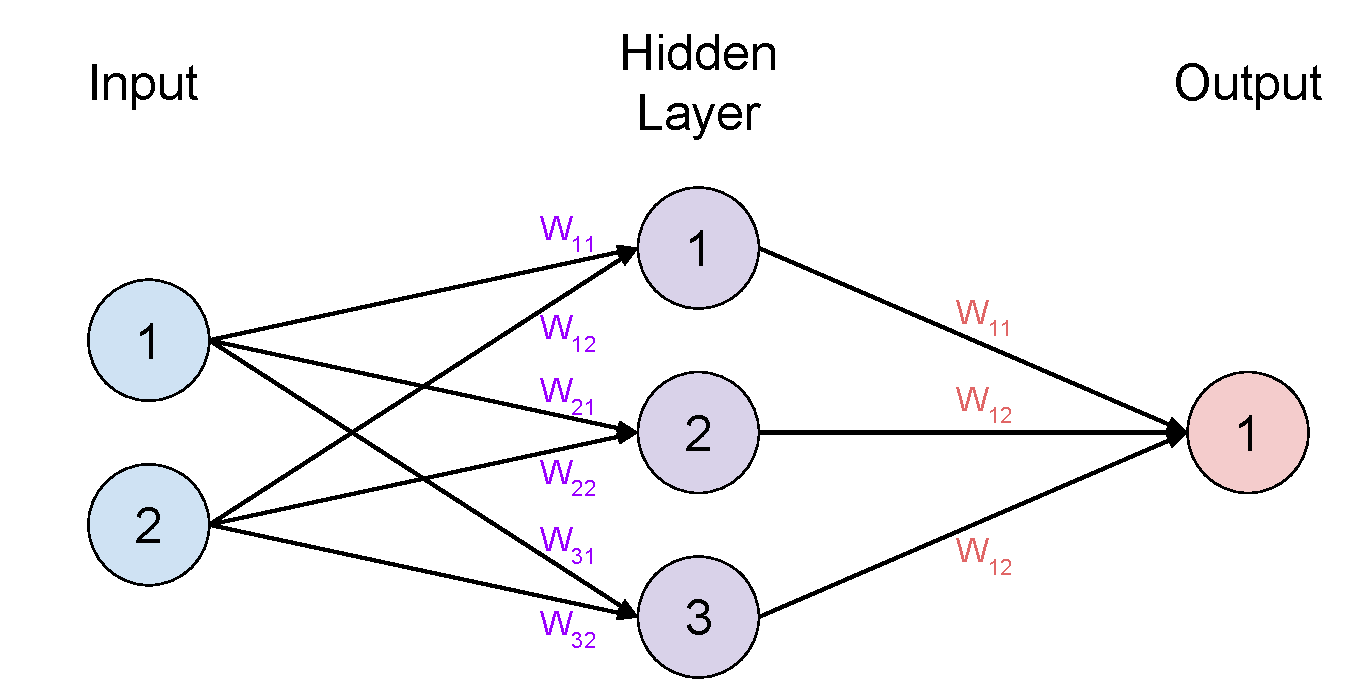
\includegraphics[width=0.8\textwidth]{simpletwolayernetwork.pdf}
	%\end{center}
	\caption{A two layer neural network with two inputs, three hidden units, and a single output. The hidden layer and output are both dense layers, and arrows depict the weighted sum computed for each unit. Weights for each layer are numbered according to their index in the weight matrix W}
	\label{fig:twolayernetwork}
\end{figure}


Despite being conceptually simple, this formulation of artificial neural networks is capable of approximating any continuous function on a compact subset in $\mathbb{R}$ with arbitrarily small error~\cite{cybenko1989}.
The challenge of using neural networks for function approximation is in finding the appropriate set of parameters to approximate the true function.
For simple feed forward neural networks, this is accomplished by quantifying the error between the true function and the approximation for a given training data set $X=(x_1, x_2, ..., x_N)$, using a differentiable loss function $L(\Theta | X)$. 
The weights are updated by differentiating $L$ with respect to $\Theta$ and "taking a step" in parameter space opposite the direction of the gradient. 
This update step can be repeated iteratively in a process called \textit{gradient descent}, which was first proposed by Augustin-Louis Cauchy~\cite{cauchy1847}.
Mathematically, 
\begin{equation}
\Theta_{k+1} = \Theta_k - \eta \nabla L(\Theta_k | X) = \Theta_k - \eta \sum_{n=1}^{N} \nabla L(\Theta_k | x_n),
\label{eq:batch_gd}
\end{equation}

\noindent
where $k$ indicates the iteration and $\eta$ is a tunable step size.
The gradient can be efficiently calculated using automatic differentiation~\cite{linnainmaa1976}, in which the update step is referred to as \textit{backpropagation}.
Weights are usually initialized by drawing from random distributions that have some empirical or theoretical justification~\cite{glorot2010}.
A variant of this algorithm, called stochastic gradient descent (SCG) performs an update using a gradient computed from a random sample of the training data at each iteration.
There is also a batched version where the training data are randomly shuffled and divided into a fixed number of equal sized \textit{mini-batches} and an update is performed on each one. 
When all mini-batches have been used in an update step, this constitutes an \textit{epoch}.
Training can be repeated for a fixed number of epochs or until the parameters sufficiently converge.
Gradient descent is a first order method, however various second order methods have also been used to train neural networks~\cite{fletcher1964, polak1969, moller1993, marquardt1963}.

Like many machine learning algorithms, neural networks risk \textit{overfitting}, in which the network learns to approximate the training data (which usually contain noise), rather than the underlying function from which the training data are assumed to be drawn.
This hinders the ability of neural networks to generalize to unseen data.
In neural networks, overfitting is commonly the result of an overcomplete parameterization coupled with overtraining~\cite{reed1993, dalianis1993}.
Many regularization techniques have been introduced to prevent overfitting of neural networks, including early stopping~\cite{morgan1990}, model pruning~\cite{reed1993}, weight decay\cite{krogh1992}, lateral inhibition~\cite{krizhevsky2012}, induced sparsity~\cite{ng2011, makhzani2015}, and dropout~\cite{srivastava2014}, with dropout being one of the most common. 
Dropout consists of randomly dropping units from the neural network during the training phase.
Each time a training example is presented to the network, each unit in the network is dropped with probability $p$, commonly 0.5.
Each application of dropout can be seen as generating a new network whose units are a subset of the units in the original network.
Given $n$ units in a network, there are $2^n$ possible dropout networks which all share weights with each other.
During testing, no dropout is performed, and weights are rescaled by $p$.
This is equivalent to averaging the prediction of each dropout network.
Dropout helps prevent overfitting by limiting the effective number of parameters in each dropout network and reducing the amount of co-adaptation among units in the network.\cite{srivastava2014}.


In recent years, more advanced forms of neural networks under the moniker \textit{deep learning} have demonstrated success in sophisticated tasks, particularly for image and speech recognition~\cite{krizhevsky2012, lecun2015, masci2011, hinton2012, he2016}, but also in a variety of other applications such as quantitative structure activity relationship (QSAR) prediction~\cite{ma2015}, particle detection~\cite{ciodaro2012}, and reinforcement learning\cite{mnih2015}.
These advances were catalyzed by the availability of large volumes of labeled data\cite{deng2009, krizhevsky2009} and the improvements in computing power from general purpose graphical processing units (GP-GPUs) and distributed systems\cite{chetlur2014, chu2007}.
Such factors allow experimentation with larger networks and more complicated layer operations such as convolutions, which are described in the following section.

\section{Convolutional Neural Networks}

Accurately labeling an image using a neural network often relies on the network's ability to detect low level features in the image such as edges and textures, which collectively indicate the an image's content~\cite{ng2011}.
This is accomplished by the appropriate set of parameters, which maximize a unit's activation when presented with a feature of interest, and can be learned through the standard backpropagation algorithm using training images. 
The challenge, however, is that the training data may not present the features of interest in all regions of the input. 
For example, suppose the labeling task is to determine if an image does or does not contain a cat.
Suppose further that no training image contains a cat in the upper left corner of the image.
Therefore it is possible, even if the network has learned which low level features indicate the presence of a cat, that it will not recognize a cat contained in the upper left corner of the image, since it has not been explicitly shown examples of this.
This may seem unlikely, but consider that the network does not incorporate any semantic meaning of the word "cat", only that a certain set of example images are positive examples and a certain set are negative examples.
Indeed, consider the slightly different labeling task where the classes being considered are "contains a cat anywhere but the top left corner" and its negation.
In this case, the same set of training images are appropriate and the hope is that the network would \textit{not} classify images with cats in the upper left corner as positive examples.
In most cases, the labeling task is more like the former example than the latter, in which case it would be beneficial for the network to learn to detect objects in a \textit{translation invariant} fashion. 
This is the primary purpose of convolutional layers.

The term convolution is inherited from the field of functional analysis, where two functions, $f$ and $g$, are combined in the following way to generate a third function, $(f*g)$:

\begin{equation}
(f*g)(t) = \int_{-\infty}^{\infty}f(\tau)~g(t-\tau)~d\tau
\label{eq:math_conv}
\end{equation}

\noindent
The convolution involves reversing one function, shifting it with respect to the other function, and integrating the product. 
Each value of $t$ represents a different relative shift.
The discrete analog of this, assuming a regularly spaced domain (in other words, a grid), takes the sum of the elementwise product of two infinite arrays.
Figure \ref{fig:cont_disc_conv} illustrates this analogy.

\begin{figure}
	\centering
	%\begin{center}
	\includegraphics[width=0.8\textwidth]{discrete_continuous_conv.png}
	%\end{center}
	\caption{The relative position of two functions at four different values of t, for both continuous (left) and discrete (right) convolutions. The functions are distinguished by color. In the continuous case, the functions are multiplied and integrated whereas in the discrete case, the elementwise product of the two arrays is taken (extending either array with zeros when necessary), and the sum of the result is taken.}
	\label{fig:cont_disc_conv}
\end{figure}

This can be extended to two dimensions by taking the sum of the elementwise product of two matrices.
Finite matrices can be considered by reinterpreting the matrices as infinite, but zero everywhere outside a finite region.
This discrete, two dimensional, finite analog to convolution forms the basis of convolutional layers in neural networks.

Consider a monochrome image as a finite matrix where the matrix entries contain pixel values in the image. 
Further, consider a smaller matrix called a \textit{filter} where the matrix entries are filter \textit{weights}.
By convolving the filter over the input image, a new matrix is created where each value is the result of summing the elementwise product of the image and filter with the filter in a particular position.
The region of the input covered by the filter is called the \textit{receptive field}, and this application of convolution can be seen as taking a weighted sum of values in the receptive field, where the weights are tied to a specific location in the receptive field.
As with dense layers, the weighted sum is typically passed through some nonlinear function before being applied to a position in the output corresponding to the filter location.
Figure \ref{fig:convolutionallayer} depicts the application of a filter to the input in a particular image.
The elementwise product naturally extends to images with multiple \textit{channels} (colors) as long as the filter has the same number of channels as the image.
The result of a convolution in a particular position depends on the values of the input image and the weights, and indeed there exist weights which produce larger outputs only in the presence of particular local features in the input.
Hence convolutions can be used in a neural network to detect patterns in the input.
Furthermore, since the same set of weights is used to convolve across the whole image, feature detection can be performed in a translation invariant way as desired. 
A filter may only detect a particular local feature, so multiple filters can be used to detect multiple features simultaneously, each producing a different channel in the output.
Note that the output of a convolution layer resembles the structure of the input, so convolutional layers may be stacked.


\begin{figure}
	\centering
	%\begin{center}
	
\includegraphics[width=0.8\textwidth]{conv_grid.png}
	%\end{center}
	\caption{Application of a 3x3 convolution filter to an input grid. The filter is multiplied elementwise with the receptive field (in green) and produces a scalar output (in red).}
	\label{fig:convolutionallayer}
\end{figure}

The design of convolutional layers gives rise to certain properties which prove useful in image related tasks:
 \begin{itemize}
 	\item \textit{Structural awareness.}
 	Convolutional filters are constructed so that they exploit the structural characteristics of the input.
 	Rather than treat each pixel of an image as independent of all others, convolutions operate on local regions of pixels, allowing filters to detect spatial correlations in a straightforward manner.
 	\item \textit{Locality}. 
 	Filters are typically significantly smaller than the size of the input, so for a given position, they are operating on a local neighborhood (receptive field) of the input image. 
 	Any features learned by a filter will necessarily be local as well. 
 	The advantage of local features is that they are simpler and more universal than global features, since they can be combined to construct a wide variety of complex patterns (see \textit{abstraction} below).
 	For example, filters which detect edges or textures will be more useful to subsequent layers in the network than a filter which recognizes only a single object or animal.
 	One exception to locality is when layers are stacked on top of one another, resulting in a larger "effective" receptive field on the original input for filters later in the network.
 	This exception is advantageous for abstraction (see below).
 	\item \textit{Translation invariance}. 
 	As discussed, a filter "inspects" each part of the image for a particular pattern, regardless of where that pattern occurred in the training images.
 	This improves generalizability because during training certain features may be presented in limited regions of the image, but detection of that feature can still operate on a global scale.
 	\item \textit{Abstraction}. Whereas a network's first convolutional layer detects patterns in the input, subsequent layers detect patterns in the output of previous layers. 
 	This promotes a hierarchical abstraction of the input, where early layers detect local features, and subsequent layers combine features into more complex patterns.
 	For example, early filters may detect edges of varying orientations, middle filters may detect combinations of edges which indicate curves in space, and latter filters may detect combinations of curves which indicate a particular handwritten letter or digit.
 	\item \textit{Resistence to overfitting}. 
 	One interpretation of a convolutional layer is that each filter is a series of units, each responsible for a distinct receptive field on the input.
 	A unit has nonzero weights only for the regions of the input in its receptive field, and all units share the same weights. 
 	This combination of weight sharing and sparsity make a convolutional layer less prone to overfitting compared to a dense layer with the same number of units.
 \end{itemize}

Convolutional neural networks often incorporate \textit{pooling layers}, which reduce a small region of the input (e.g. 2x2 pixels for an image) to a single grid element that takes either the maximum or average value (per channel) of the region. 
Pooling allows downsampling of the grid, and is often performed between convolutional layers. 
It's also common to include a series of dense layers after all convolutional layers which combine the results of convolution in a way relevant to the learning task.
Because of the weight sharing in convolutional layers, the final dense layers often contain the majority of the parameters in the network.


 The above properties make convolutional neural networks well suited for structured data with a natural hierarchy of abstraction.
 The structural hierarchy of proteins suggests that convolutions might be useful in interface prediction.
 Unfortunately, neither protein residues, nor their constituent atoms are aligned in a regular grid, so the above definition of convolution cannot be directly applied. 
 In Chapter \ref{chap:methods}, new convolutions are introduced which operate on irregular structures, namely graphs, and a graphical model of proteins is presented which allows use of these graph convolutions for protein interface prediction.

%\chapter{Pairwise Graph Convolutional Networks for Interface Prediction}
\label{chap:methods}

The methods presented in this thesis were motivated by a desire to exploit the local structure around a residue when performing interface prediction.
The biological reasoning for this is that a residue's neighborhood influences its propensity to participate in an interface.
It was noted in Chapter \ref{chap:neuralnetworks} that convolutional neural networks are one way of detecting features in a local neighborhood, but they are limited to regular grids. 
Unfortunately, proteins cannot naturally be represented as a regular grid, so convolution must be developed for a more natural representation: graphs.


\section{Proteins As Graphs}

An undirected, unweighted graph $G$ consists of a set of vertices, $V=\{v_1, v_2, ..., v_n\}$, and a set of eges, $E=\{e_1, e_2, ..., e_m\}$ where each edge is incident to two vertices and there is at most one edge between two vertices.
One way of representing proteins as graphs is to let each vertex represent a residue in the protein, and each edge represent the relationship between two residues.
Thus any information pertaining to a particular residue can be associated with the relevant vertex in the form of a feature vector.
The features used in this work are drawn from features used in prior interface prediction work \cite{minhas2014}.
Likewise, any information about the relationship between two residues can be associated with the relevant edge.
The edge features used here describe the distance between and relative orientation of two residues.
These edge features are defined between any two residues in the protein, so the graph is complete. 
A detailed explanation of each feature is contained in Appendix \ref{appendix:features}.

This representation is an abstraction of the original protein to a well studied mathematical object, with two notable facts.
First, the graph itself does not rely on a coordinate system, as is the case when working with raw 3D positions.
Second, the features contained on the graph are also not tied to a coordinate system.
This is because they either describe coordinate free attributes of individual residues, or they describe relative spatial relationships between two residues.
These facts make a protein graph invariant to rotations or translations in space.
However, since the graph was constructed from points in 3D space, local neighborhoods of vertices can be defined using spatial proximity.
This is useful when designing convolutions that use a local neighborhood as a receptive field.
With proteins represented as graphs, the remaining task is to design a convolution which operates on graphs. 

\section{Graph Convolution}
Recent years have seen increased attention to problems involving graph structured data, prompting developments in graph convolution to perform various tasks on those data~\cite{bronstein2016}.
These developments allow leveraging of deep learning techniques, which have shown great success for problems on regular grids.
Though each variant of graph convolution is tailored to suit the data and problem being addressed, there are some common approaches which merit describing generally.
These approaches generally fall into one of two categories: \emph{spectral} or \emph{spatial}.


\subsection{Spectral and Spatial Graph Convolution}
Spectral methods of graph convolution are based on linear functions in the frequency domain of a graph, defined using the laplacian operator $\mathcal{L}=I-D^{-1/2}WD^{-1/2}$, where $I$ is the identity matrix, $W$ is a matrix of edge weights, and $D$ is a diagonal matrix containing the degree of each vertex~\cite{bruna2013, henaff2015, kipf2016}.
Each filter in a spectral convolution implies a weighting of each frequency in the spectral decomposition of the graph~\cite{mallat2009}.
In physics, the Laplacian operator is used to model the process of diffusion.
In a similar way, the graph Laplacian can be thought of as modeling diffusion along the edges of the graph.

Spatial approaches instead define operations in a localized neighborhood of a central vertex~\cite{henaff2015, atwood2016}.
Each neighborhood constitutes a receptive field where a convolution operation is performed (see Figure \ref{fig:spatial_graph_conv}).
Spatial convolution commonly involves a vector of weights and takes a weighted sum of neighbors, much like a discrete convolution on a grid can be viewed as taking a weighted sum of pixels within the receptive field.
Spatial convolution is more directly analogous to grid based convolution as described in Chapter \ref{chap:neuralnetworks}.
There is a critical difference, however, in that receptive fields from different parts of a graph have no natural correspondence with one another.

\begin{figure}
	\centering
	%\begin{center}
	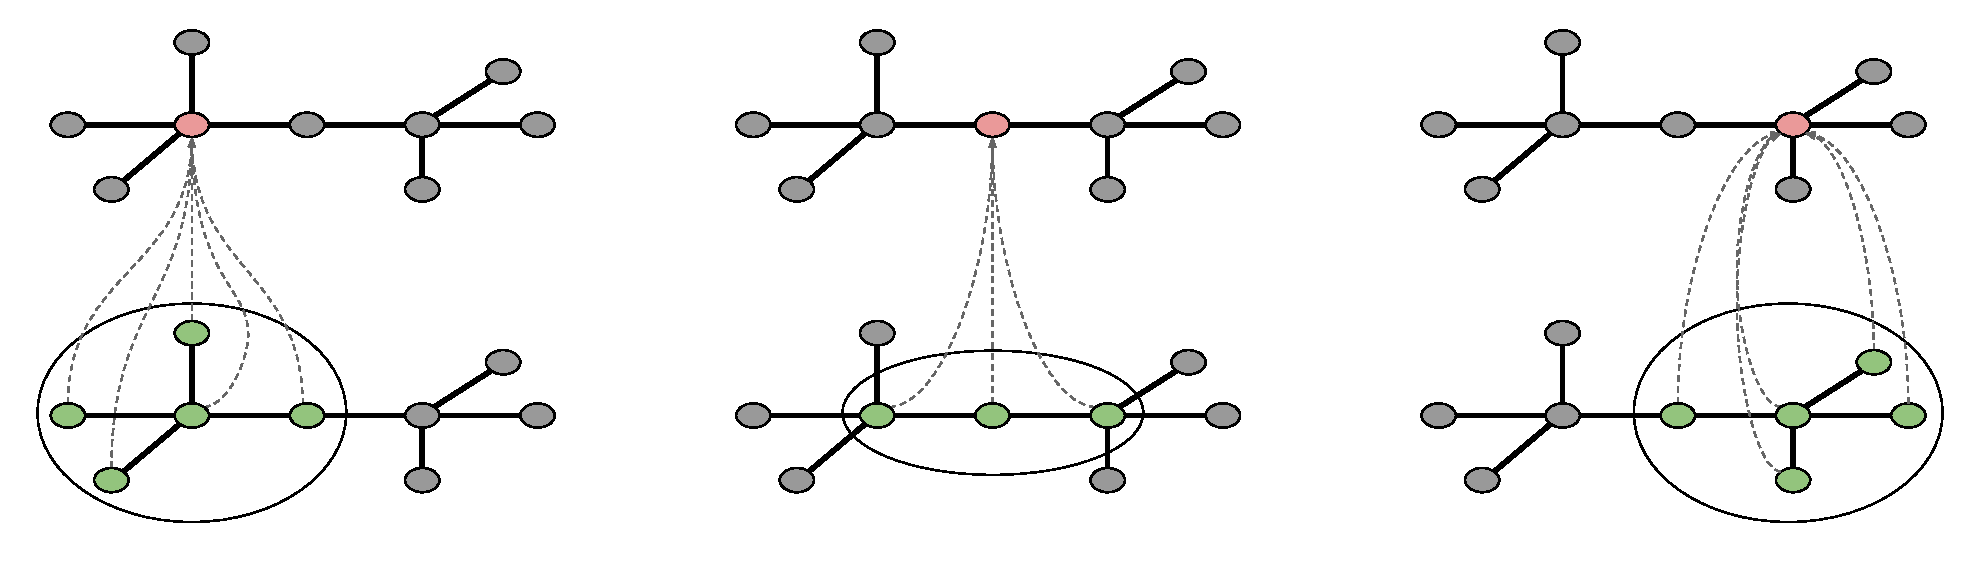
\includegraphics[width=\textwidth]{conv_graph.pdf}
	%\end{center}
	\caption{Receptive fields in a graph context, where each receptive field is defined around a central vertex. The result of convolution is applied to the central vertex in the receptive field.}
	\label{fig:spatial_graph_conv}
\end{figure}

\subsection{Receptive Field Correspondence in Spatial Convolution}


Grid receptive fields have defined positions, such as "upper left most" or "bottom middle".
Therefore weights can be applied consistently across receptive fields such that each weight is always applied to the same position.
With graphs, there is often no such correspondence between receptive fields, since vertices are inherently unordered and lack a specific position (recall their coordinate free nature).
The only well defined position is the center, but the problem remains with the neighbors.
In fact, the number of neighbors may vary from one receptive field to another, depending on the definition of a local neighborhood.
Figure \ref{fig:grid_vs_graph_rf}
Hence the consistent application of weights across receptive fields is only possible after these issues have been addressed.
This is typically done in one of two ways:

\begin{figure}
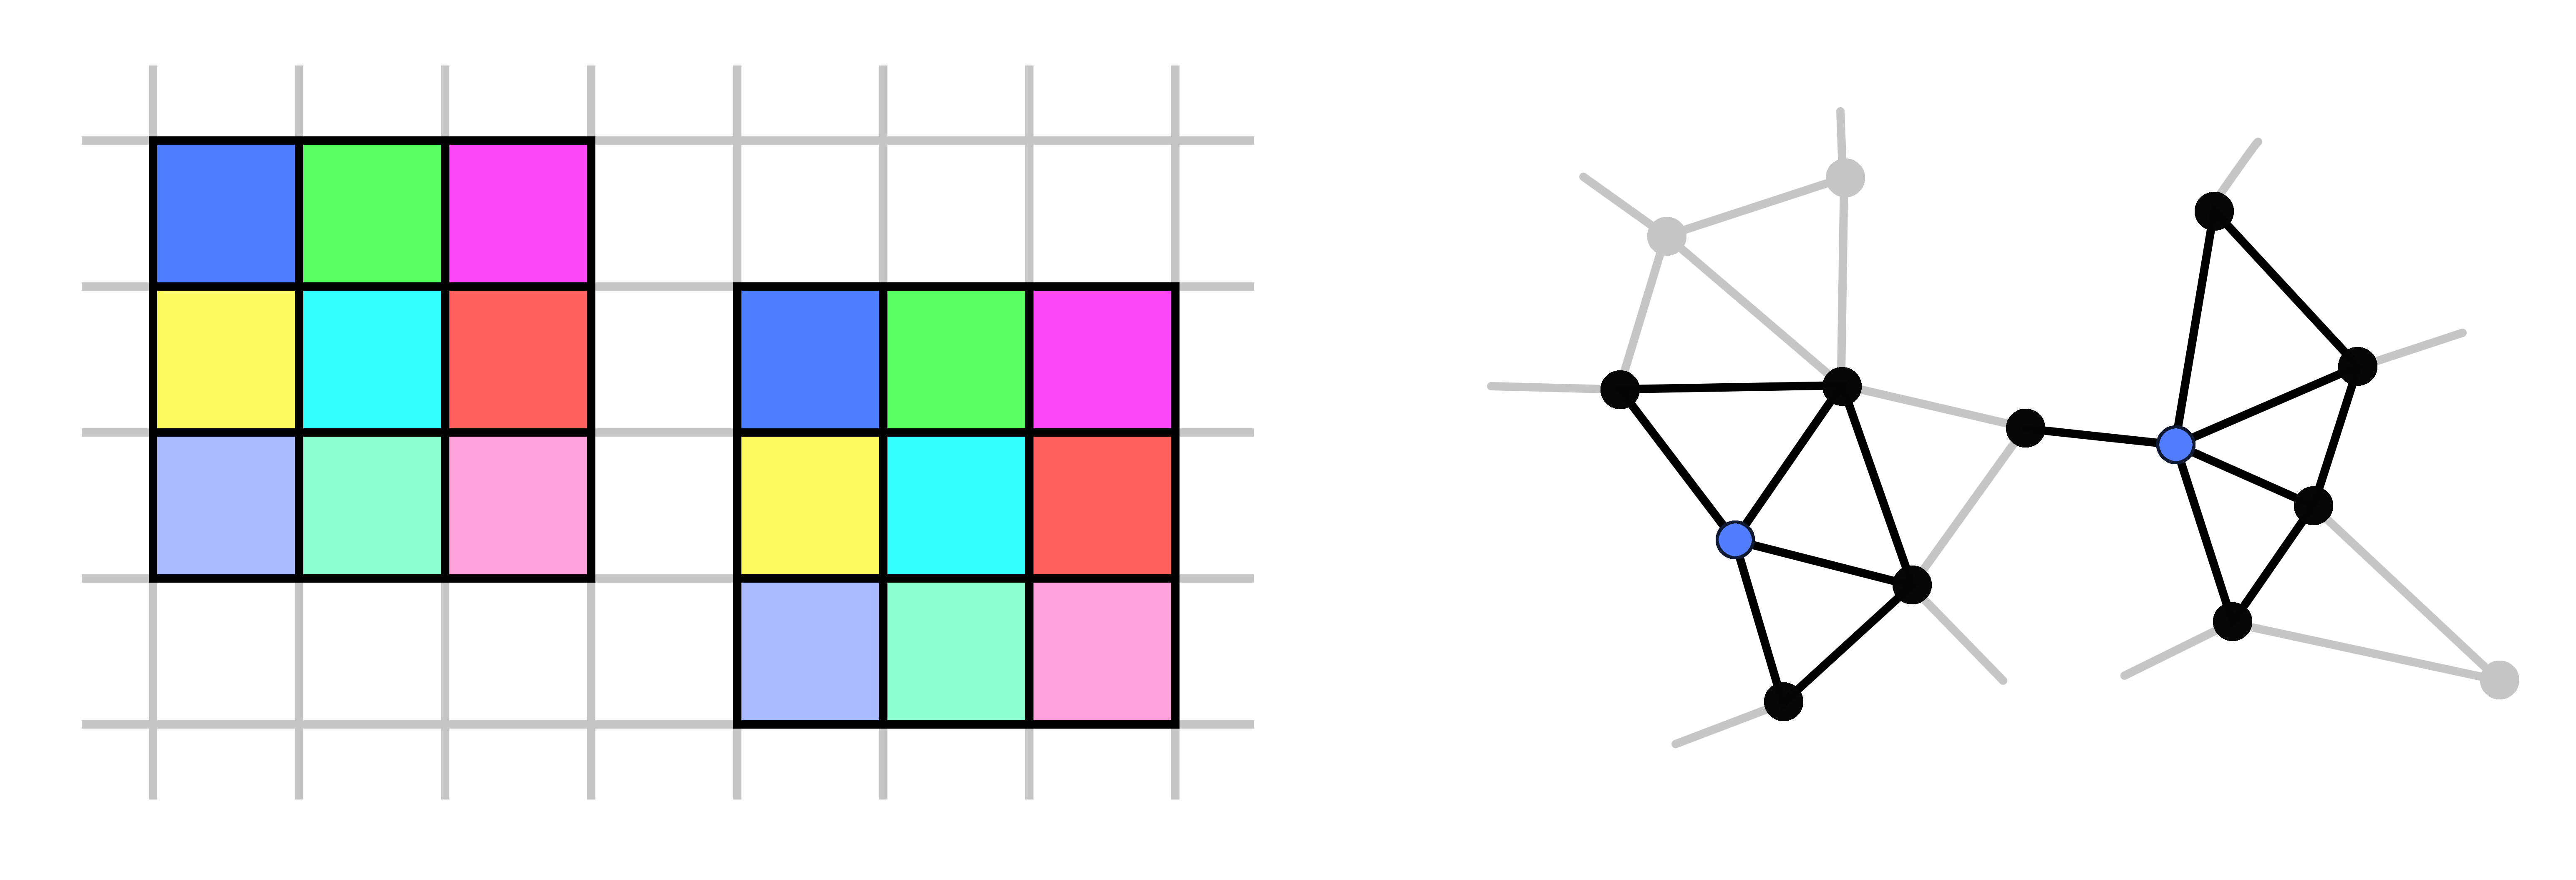
\includegraphics[width=0.9\textwidth]{grid_vs_graph_rf.png}
\caption{The difference between grid receptive fields and graph receptive fields. Grid receptive fields give rise to positions (denoted by color) which are consistent from one receptive field to another. Graphs have no set positions other than the central vertex (in blue).}
\label{fig:grid_vs_graph_rf}
\end{figure}

\begin{enumerate}
	\item \textit{Imposed ordering of neighbors}. This approach establishes a correspondence between two receptive fields by ordering the neighbors in each and associating neighbors sharing a common position. 
	Ordering methods are either based on vertex characteristics, like degree and betweenness centrality, or domain specific knowledge ~\cite{niepert2016, duvenaud2015}.
	They typically require the number of neighbors in a receptive field to remain the same.
	This approach allows filter weights which are applied to a particular position in the ordering, which, it is assumed, has some significance across all receptive fields.
	If the imposed ordering is arbitrary, this approach has limited usefulness.
	Methods following this approach can be called \emph{ordered}.
	
	\item \textit{Identical treatment of neighbors}. This approach ignores the need to establish a correspondence between receptive fields and instead treats all neighbors identically.
	Rather than apply different weights to neighbors depending on their position in an ordering, the same weights are applied to each neighbor.
	This allows for different sizes of receptive fields and avoids choosing an ordering method, but lacks the ability to treat each neighbor uniquely.
	Methods following this approach can be called \emph{order free}.
\end{enumerate}

Figure \ref{fig:correspondence_approaches} depicts both approaches.
Examples of each were evaluated for this thesis.
In addition, novel convolutions were examined which attempt to incorporated the advantages of both ordered and order free methods.
Below is a description of each existing method followed by the novel methods presented in this thesis. 

\begin{figure}
	\centering
	%\begin{center}
	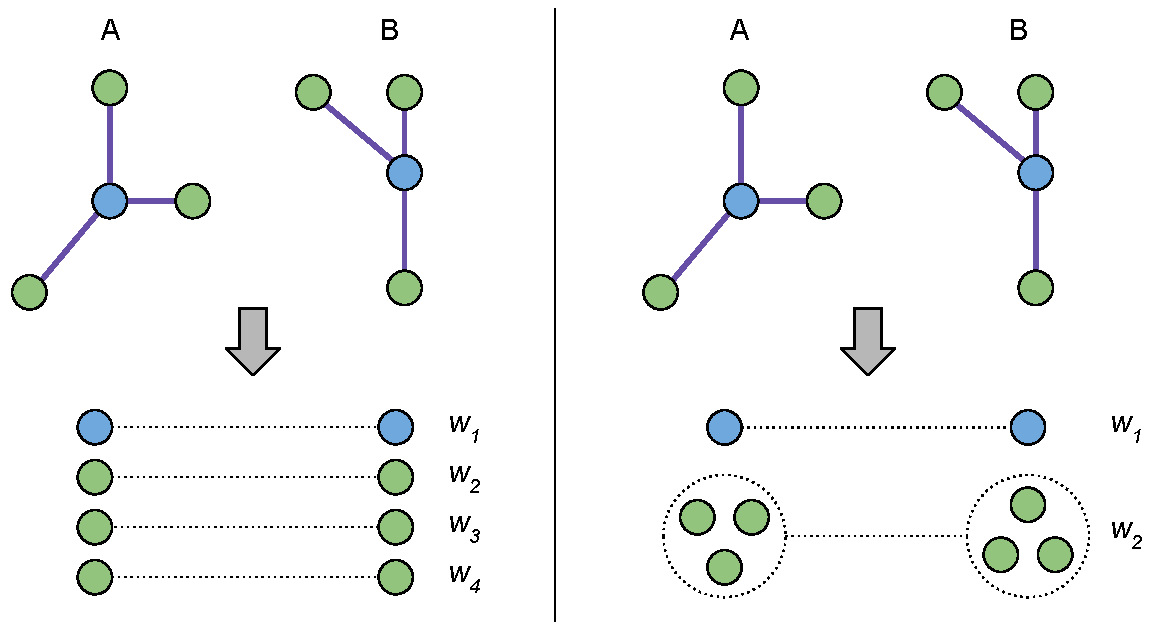
\includegraphics[width=0.8\textwidth]{correspondence_approaches.pdf}
	%\end{center}
	\caption{Two approaches of establishing correspondence between the neighbors of receptive fields A and B. Central vertices are shown in blue and neighbors in green. The central vertices always correspond with one another. Left: neighbors are ordered and placed into correspondence based on position. Unique weights (\textit{$w_2$--$w_4$}) can then be applied to each position in the order. Right: neighbors are left unordered and treated identically. This requires that the same weights (\textit{$w_2$}) be used for all neighbors.}
	\label{fig:correspondence_approaches}
\end{figure}


\subsection{Diffusion Based Method}
As mentioned, spectral methods utilize the Laplacian operator, which is used to model diffusion processes. 
Although no spectral methods were examined in this thesis, a non-spectral diffusion method was.
Atwood \& Towsley~\cite{atwood2016} propose a Diffusion Convolutional Neural Network (DCNN) which uses a graph's weight matrix as a transition matrix by normalizing rows.
The transition matrix $P$ is raised to successive exponents, generating a power series, with each power corresponding to all walks of length equivalent to that power.
For a maximum power of $L$, the activation of a node is:

\begin{equation}
h(x_i | W) = \sigma \bigg( \sum_{l=0}^L (W_{l\cdot} \odot P^l X ) \bigg),
\label{eq:diffusion}
\end{equation}

\noindent
where $W$ is a matrix of weights, $W_{l\cdot}$ is its $l^{th}$ row, $\odot$ denotes broadcasted elementwise multiplication, and $X$ is a matrix of all vertices, where each row is a vertex and each column a different feature.
For each power $l$, all vertices that have a random walk of length $l$ that end at the vertex of interest are summed together, weighted by the walk probability.
This sum is then multiplied elementwise with a weight vector and summed with the result of all other powers to produce the overall signal.
Unlike other convolutions presented here, this method does not use a receptive field, instead relying on the similarity matrix to indicate proximity.


\subsection{Ordered Method}

Niepert, Ahmed, \& Kutzkov~\cite{niepert2016} describe an ordered graph convolution that is used in their tool, \emph{PATCHY-SAN}, which performs classification at the graph level.
This methods constructs local neighborhoods orders neighboring vertices according to a \emph{normalization} procedure.
The ordered vertices serve as the receptive field for convolution at the central vertex, which is also in the ordering. 
If $(x_1, x_2, ... , x_k)$ is the ordered list of vertices, then convolution takes the form:

\begin{equation}
h(x_i | \{ W_{j} \}, b)= \sigma \bigg( \frac{1}{k} \sum_{j=1}^{k}(W_{j} x_j) + b \bigg),
\label{eq:patchysan}
\end{equation}

\noindent
where $W_j$ is the weight matrix for position $j$ in the ordering.
A natural ordering technique is one which places the center vertex first and orders its neighbors from least to greatest distance from the center. 
In this way, one weight matrix is used for all center vertices, another for all nearest neighbors, etc.
The vertex ordering also imposes a lexicographic ordering on the neighborhood edges as well, so unique weights can be used to generate a signal from each edge. 
Adding this term to the convolution generates:

\begin{equation}
h(x_i | \{ W_{j} \}, \{ W_{jk} \}, b)= \sigma \bigg( \frac{1}{k} \sum_{j=1}^{k}(W_{j} x_j) + \frac{1}{k^2} \sum_{j = 1}^{k-1} \sum_{l=j+1}^{k}(W_{jk} A_{jk})  + b \bigg),
\label{eq:patchysan_2e}
\end{equation}

\noindent
where $W_{jl}$ is the weight matrix associated with edge $(j, l)$ in the lexicographic ordering.
Originally, Niepert et al. convolve vertices and edges separately and combine them in a subsequent layer.
Classification is then performed on the whole graph level.
For interface prediction however, the edges and vertex signals are averaged together and applied to the central vertex so that repeated graph convolutions may be performed without losing the graph structure, and no graph labeling is necessary.
Within a receptive field, vertices are ordered based on the residue's distance from the residue of interest.

\subsection{Order Free Methods}
One of the simplest forms of order free graph convolution was proposed by Duvenaud \& Maclaurin, et al.~\cite{duvenaud2015}, which was used for generating molecular \emph{fingerprints}.
This method uses a single set of weights for all vertices in the receptive field, including the central vertex:

\begin{equation}
h(x_i | W, b)= \sigma \bigg( W x_i +  \frac{1}{|\mathcal{N}_i|} \sum_{j \in \mathcal{N}_i} (W x_j) + b\bigg),
\label{eq:fingerprint}
\end{equation}

\noindent
where $\mathcal{N}_i$ is the index set of all neighbors of $x_i$.
In the original formulation, no bias term was included, and the sum was not divided by the neighborhood size.
However, when used for interface prediction, including the bias and normalization provided better overall results.

As mentioned, center vertices may be treated separately from the neighbors, even if all neighbors are treated identically. 
Schlichtkrull \& Kipf~\cite{schlichtkrull2017} proposed such an approach called \emph{Relational Graph Convolutional Networks}, or R-GCN.
Their methods were developed for use in knowledge bases, graph structures where the vertices are named entities and the edges capture the many binary relationships between the entities. 
To convolve a vertex, they take the neighborhood defined by each relation type and sum the signal from all the neighbors in that neighborhood.
The resultant signal is the sum of signals from each relation type.
For protein graphs, spacial proximity is the only method for determining neighborhoods that makes sense biologically, so there is only one neighborhood.
The adapted version of this convolution for use in interface prediction is:

\begin{equation}
h(x_i | W^\textsc{c}, W^\textsc{n}, b)= \sigma \bigg( W^\textsc{c} x_i + \frac{1}{|\mathcal{N}_i|} \sum_{j \in \mathcal{N}_i}(W^\textsc{n} x_j)  + b\bigg),
\label{eq:rgcn}
\end{equation}

\noindent
where separate weight matrices, $W^\textsc{c}$ and $W^\textsc{n}$, are used for the center and neighbors, respectively
In the original version, a different weight matrix was used for each of the many relation types.  
To reduce the number of model parameters to tie learning across all relation types, all weight matrices were simply linear combinations of a set of learnable basis weight matrices:

\begin{equation}
\begin{split}
W^\textsc{n} = \sum_{b} a^\textsc{n}_b V_b \\
W^\textsc{c} = \sum_{b} a^\textsc{c}_b V_b 
\end{split}
\label{eq:rgcn_basis}
\end{equation}

\noindent
where $\{V_b\}$ is a set of basis functions, $a^\textsc{c}$ and $a^\textsc{n}$ are scalar weights that combine the basis functions to create $W^\textsc{c}$ and $W^\textsc{n}$, respectively.
For interface prediction, R-GCNs were examined with and without basis functions.

The above order-free methods do not incorporate edge information.
Sch{\"u}tt, Arbabzadah, Chmiela, M{\"u}ller, \& Tkatchenko~\cite{schutt2017} propose a version called \emph{Deep Tensor Neural Networks} (DTNN) which creates a signal for the neighbor vertices as well as the edges which connect them to the central vertex:

\begin{equation}
h(x_i | W, W^\textsc{n}, W^\textsc{e}, b^\textsc{n}, b^\textsc{e})= x_i + \frac{1}{|\mathcal{N}_i|} \sum_{j \in \mathcal{N}_i} \sigma \bigg[ W \bigg( (W^\textsc{n} x_j + b^\textsc{n}) \odot (W^\textsc{e} A_{ij} + b^\textsc{e}) \bigg) \bigg],
\label{eq:deep_tensor}
\end{equation}

\noindent
where $A_{ij}$ are the features for edge $(i, j)$, and $\odot$ denotes the elementwise product.
In this formulation, $W^\textsc{n}$ and $W^\textsc{e}$ transform vertices and edges respectively into a common space, and $W$ transforms their combination back into the dimensionality of the input. 
This convolution does not transform the input by any weight matrix, rather it can be viewed as updating the representation at $x_i$ using information from its neighbors.
This restricts representations to always have the same dimensionality, which is not generally required in convolutions. 
Again, the normalization is omitted from the original formulation, but consistently improves performance.
Ideally, the central vertex would have a weight matrix.
Nevertheless, this method uniquely incorporates edge information, so that even while all neighbors use the same weight matrix, the information on their edges is used to differentiate them.
This concept is carried forward into the convolution methods proposed below.


\subsection{Proposed Order-Free Methods}
Like DTNN, these methods incorporate edge information to help differentiate neighbors, but also avoid imposing an arbitrary ordering on the neighbors in a receptive field.
This is accomplished by incorporating information from the edges between each neighbor and the central vertex.
Here are two variants of graph convolution which differ only in how the edge information is incorporated, denoted \textit{Sum Coupling} and \textit{Product Coupling}.
For a central vertex $i$ on the graph and a local neighborhood of vertices $\mathcal{N}_i$, the output of \emph{Sum Coupling} graph convolution is:
\begin{equation}
h(x_i | W^\textsc{c}, W^\textsc{n}, W^\textsc{e}, b) = \sigma \bigg( W^{\textsc{c}} x_i + \frac{1}{|\mathcal{N}_i|}\sum_{j \in \mathcal{N}_i} (W^{\textsc{n}} x_j + W^{\textsc{e}} A_{ij}) + b \bigg),
\label{eq:sum_coupling}
\end{equation}
where $x_i$ is the feature vector associated with vertex $i$, $A_{ij}$ is the feature vector associated with edge $(i, j)$, $W^\textsc{c}$, $W^\textsc{n}$ and $W^\textsc{e}$ are weight matrices, and $b$ is a vector of biases. 
If there are $l$ vertex channels, $p$ edge channels, and $k$ filters, then $W^\textsc{c}\in\mathbb{R}^{k \times l}$, $W^\textsc{n}\in\mathbb{R}^{k \times l}$, $W^\textsc{e}\in\mathbb{R}^{k \times p}$, and $b\in\mathbb{R}^{k}$.
Intuitively, this calculates an activation for the central vertex, each neighbor vertex, and each edge between a neighbor and the central vertex separately.
It is the inclusion of edge activations that allows each neighbor to be distinguished from the others on the basis of its relationship to the central vertex.
This variant is called Sum Coupling because the neighbor vertex and edge activations are added together.
Because of this, the direct association between a neighbor its edge is lost.
A variant which maintains the association is \emph{Product Coupling}, whose output is:
\begin{equation}
h(x_i | W^\textsc{c}, W^\textsc{n}, W^\textsc{e}, b) = \sigma \bigg( W^{\textsc{c}} x_i + \frac{1}{|\mathcal{N}_i|}\sum_{j \in \mathcal{N}_i} (W^{\textsc{n}} x_j \odot W^{\textsc{e}} A_{ij}) + b \bigg),
\label{eq:prod_coupling}
\end{equation}
where $\odot$ denotes the elementwise product between two vectors or matrices. 
This allows a neighbor's influence on the overall activation to be modulated by its relationship to the central vertex.
For protein graphs, this means neighboring residues will contribute more or less to the overall activation, depending on their distance from and relative orientation to the central vertex, with the precise modulation determined by the edge activations.
Note the similarity to Equation (\ref{eq:deep_tensor}).

Just as convolution on a regular grid can be applied at any pixel in an image, graph convolution can be applied to any vertex in the graph.
Hence both can be considered translation invariant.
Both Sum Coupling and Product Coupling graph convolution are translation invariant, don't impose an ordering on the neighbors or a correspondence between receptive fields, allow for different numbers of neighbors, and account for the different relationships between neighbors and the central vertex. 
The receptive fields are always defined around a central vertex, so the results of convolution can be applied to that vertex.
This retains the graph structure after each convolution, so convolutional layers are stackable, as with images.

A note on receptive fields: protein graphs are complete and embedded in a metric space, so this thesis defines a receptive field using a fixed number of closest neighbors to the central vertex.
A receptive field can also be defined using a threshold $\delta>0$ such that all vertices closer to the central vertex than the threshold are included in the receptive field.
All neighbors in a receptive field are guaranteed to share an edge with the central vertex, allowing the application of equations (\ref{eq:sum_coupling}) and (\ref{eq:prod_coupling}).
For incomplete graphs, a receptive field can be defined as all vertices within $k$ hops of the central vertex. 
If $k=1$, both versions of graph convolution can directly be applied.
If $k>1$, then Product Coupling graph convolution can't be directly applied to neighbors more than 1 hop away from the center vertex, since they share no edge with the center. 
Though there are ways to adapt Product Coupling graph convolution in this situation, they are not the focus of this thesis.
%TODO: say more?

Lastly, to assess the benefit that incorporating information from neighboring residues has on classification performance, the \emph{no convolution} variant is defined as:

\begin{equation}
h(x_i | W^\textsc{c}, b)= \sigma \bigg( W^{\textsc{c}} x_i + b \bigg),
\label{eq:no_conv}
\end{equation}

\noindent
which resembles the activation of a dense layer in regular neural networks.


\section{Pairwise Neural Network Architecture}
These graph convolution operations allow the detection of local patterns on a single graph, and produce a new representation at each vertex.
Partner specific protein interaction, however, requires classifying pairs of residues in different proteins (vertices in different graphs), which is essentially making predictions on vertices in the product graph. 
Such predictions are made using a pairwise neural network architecture.

A pairwise architecture consists first of two identical convolutional modules, each responsible for generating the representation for one of the proteins in the pair.
A key requirement for the pairwise architecture is symmetry, since the prediction for a pair of residues should be the same irrespective of which leg is used for each protein.
To ensure symmetry in the convolution layers, weights are shared between layers in the different legs.
The merge layer then combines the vertex representations from one graph with the vertex representations from the other into pairs.
To maintain symmetry, this merge process should also be symmetric.
For example, the elementwise sum, elementwise product, and outer-product are all commutative and therefore produce symmetric output.
Another option is to combine pairs asymmetrically, such as concatenating the two representations together, but then average the predictions from each ordering of the representations.
%TODO: talk about pairwise kernels?
Finally, the combined representation for each pair of residues is passed through a number of fully connected layers.
The data are represented as pairs of residues at this point. 
Theoretically, graph convolution could be performed at this stage as well, this time in the product graph.
However, the computational and memory requirements of doing so prove prohibitive since the number of convolutions and the number of neighbors in each convolution increases quadratically.
Hence the work in this thesis performs no convolution after merging.
The final layer has a single output for each pair indicating the prediction for that pair.
See Figure \ref{fig:pairwise_arch1} for a graphical depiction.

This output is converted to a binary class prediction vector using a softmax function, 

\begin{equation}
\text{softmax}(x) = \bigg[ \frac{e^{-x}}{e^{x} + e^{-x}} , \frac{e^{x}}{e^{x} + e^{-x}} \bigg],
\label{eq:softmax}
\end{equation}

\noindent
the elements of which can be interpreted as class probabilities for the negative (non-interfacial) and positive (interfacial) classes, respectively.
This output is compared to a one-hot label vector indicating whether \big($[0, 1]$\big) or not\big($[1, 0]$\big) the pair constitute part of the true interface. 

\begin{figure}
	\includegraphics[width=\textwidth]{pairwise_network4.pdf}
	\caption{A pairwise neural network architecture that takes two protein graphs as input. Each leg contains one or more convolutional layers. The resultant graphs are then merged to create representations of residue pairs. After more fully connected layers, a final classification is performed for each pair.}
	\label{fig:pairwise_arch1}
\end{figure}


This chapter has presented protein graphs, graph convolution operations, and pairwise neural network architectures, all of which are components in this deep learning approach partner specific protein interface prediction.
Chapter \ref{chap:experiments} describes the experiments that were performed and gives a discussion of the results.


%\chapter{Experiments}
\label{chap:experiments}

The proposed pairwise graph convolutional neural networks were evaluated and compared to prior work in both partner specific interface prediction and graph convolution.

\section{Data}

Each model was trained, validated, and tested using complexes from the Docking Benchmark Dataset (DBD) version 5.0~\cite{vreven2015}, a collection of 3D crystalline structures of transient complexes in both the bound and unbound formations. 
DBD is non-redundant in the sense that no two proteins in one complex are in the same Structural Classification of Proteins (SCOP)~\cite{murzin1995} families as two proteins in another complex, respectively.
This ensures the dataset is appropriate for testing since methods that perform better on certain SCOP families than others are not unfairly rewarded or penalized.
Each protein is classified into either \emph{rigid body}, \emph{medium difficulty}, or \emph{difficult}, based on the degree of conformational change of the interfaces.
This is quantified using the root mean squared deviation of the alpha carbons after unbound and bound structures are superimposed on one another. 
Training and validation were performed using the 175 complexes that were present in version 4.0 of DBD, whereas the 55 new complexes added in DBD 5.0 were reserved for testing. 
Training and validation sets were created using a 80\%/20\% partition on the DBD v4.0-only complexes, such that the class proportions in each partition were roughly equivalent.
Hence there were 140 training complexes and 35 validation complexes.
Table \ref{tab:examples} indicates the number of positive and negative examples used from each dataset.

\begin{table}
	\centering
	\begin{tabular}{l l c r r}
		\toprule
		Phase & Data Set & Complexes & Positive examples  & Negative examples \\ 
		\midrule
		\multirow{2}{*}{Model Selection} 
			& Train      & 138       & 12,632 (9.1\%)     & 126,320 (90.9\%) \\
			& Validation & 34        & 3,042 (0.2\%) 		& 1,868,270 (99.8\%) \\
		\midrule
		\multirow{2}{*}{Testing}
			& Train + Validation & 175 & 16,004 (9.1\%) & 160,040 (90.9\%) \\
			& Test       & 55        & 4,871 (0.1\%)      & 4,953,446 (99.9\%) \\ 
		\bottomrule
	\end{tabular}
	\caption{Number of complexes and examples (residue pairs) for each phase of experimentation. Negative examples were down sampled to a ratio of 10:1 with positive examples when training, but testing included all examples. During model selection, three complexes were excluded from the training and validation sets due to a software bug and missing features. These complexes were eventually included for the testing phase. \label{tab:dataset_size}}
	\label{tab:examples}
\end{table}

3D structures are contained in Protein Data Bank (PDB) files, which contain atomic coordinates for each amino acid in the complexes.
True interfaces were determined using the bound formations, where two amino acids are assumed to be interacting if they are within 6 \AA{} of each other, in consistent with prior work~\cite{ofran2007, ahmad2011, minhas2014}.
This permits an amino acid residue to interact with multiple partners in the interface.

\subsection{Vertex and Edge Features}
Prediction must be made using the unbound formation of each protein, since the bound formation is not known a priori.
Hence unbound PDB files were used to generate a graph representation of each protein, with vertices indicating residues and edges indicating the relationships between residues.
Features were then computed for each vertex and edge using sequence and structure information from the protein.
Vertex features pertain to the degree of residue conservation, accessible surface area, depth within the protein, and protrusion.
Edge features capture the distance between two residues and their relative orientation as well.
More detail on each feature can be found in Appendix \ref{appendix:features}.

\subsection{Missing Data}
In some cases, features could not be calculated for a residue, resulting in missing values.
For 13 residues, the atomic coordinates of the central alpha carbon were not present in the PDB files, so the Half Sphere Amino Acid Composition, Residue Depth, and $\mathrm{C C_{\alpha} O}$ angle could not be calculated.
Most features rely on third party software to calculate the features from the raw sequence and structure information.
For the proteins with DBD codes 2B42 and 3R9A, features related to the protrusion index could not be calculated for the receptor due to a software fault.
These complexes were omitted during model selection but re-introduced before testing.
Two other complexes, 1NW9 and 1PPE, were also excluded during model selection due to a software bug.
This bug was eventually fixed, so these were also included during testing. 
During model selection, missing values were imputed using the feature mean within a proteins, whereas for testing, the global median (within the training, validation, or test set) was used.
In total there were 138 training and 34 validation complexes during model selection, and there were 175 training and 55 test complexes during testing.
%TODO: find total number of nans?

\section{Experiments}

Experimentation was conducted in two phases: model selection, and testing.
The model selection phase concerned the selection of model \emph{hyper-parameters}, those details which are not explicit model parameters but nevertheless affect the behavior of the network.
For this phase, pairwise graph convolutional networks were repeatedly trained using the training set and evaluated on the validation set.
Once model selection was complete, the final set of model hyper-parameters was used to train and test the most promising hyperparameter configurations and compare them to existing methods.
For this phase, the model was trained on the combined training and validation sets and tested on the test set.


\subsection{Model Selection}

Not only do a network's parameters ($\Theta$) help determine the network's output, but the set of hyper-parameters as well.
Hyper-parameters comprise all model specifications besides the parameters themselves, such as the number and types of layers, number of units/filters in each layers, choice of nonlinear activation function, loss function, and training details.
Hyper-parameters are typically chosen either by some automated process, or by manual exploration.

Automated hyper-parameter selection processes include a randomized search, grid search, or a sequential, model based optimization (SMBO) algorithm such as a Gaussian Process or Tree Structured Parzen Estimator~\cite{bergstra2011}.
The advantage of these approaches is their ability to automatically search a hyper-parameter space without human intervention. 
SMBO approaches are able to estimate the performance "response surface" in hyper-parameter space in order to efficiently find the optimum value.
The disadvantage of these approaches is they sometimes require a large number of iterations in order to converge to optimal parameters, and it may be difficult to incorporate human prior knowledge about the optimal set of hyper-parameters.
Some experiments were performed with SMBO algorithms, but none produced hyper-parameters which outperformed results found by human exploration.
One hindering factor for the automated approaches was the sheer number of parameters being explored, making it difficult to sample the space in an efficient way.
%TODO: report number of hyperparameters tried?
Therefore automated approaches were abandoned in favor of a manual search.

Several hyper-parameters were explored manually by training/validating networks under different settings of the hyper-parameters.
This exploration occurred in a one-hyper-parameter-at-a-time fashion, alleviating the exponential problems encountered with the automated algorithms, but also limiting the ability to explore the interactions between different hyper-parameters.
Following is a list of different hyper-parameters which were explored and the general trends encountered in each.
\begin{itemize}
	\item Number of convolutional layers:
	\item Number of convolution filters:
	\item Receptive field size:
	\item Number of dense layers after merge:
	\item Parameter inizialization: weights and biases
	\item Nonlinear activation function:
	\item 
	\item Loss function:
	\item Update algorithm:
\end{itemize}

The cumulative findings of and intuition gained from the manual model selection procedure informed the final set of experiments which were run in the testing phase of experimentation.

\subsection{Testing}

Final model testing was performed for both sum coupled and product coupled graph convolutions.
For each variant, receptive field sizes of 11 and 21 were tested (the central vertex plus 10 or 20 neighbors, respectively), with one, two three, and four graph convolutional layers. 
In total, 16 hyper-parameter conditions were tested, all of which used the following training scheme:
The number of filters for networks with one convolutional layer was 256, Likewise for two, three, and four convolutional layers the number of filters was (256, 512), (256, 256, 512), and (256, 256, 512, 512) respectively. 
After merging examples, dense layers of 256 and 1 units respectively were applied, with the latter producing the model output.
Loss was computed using weighted cross entropy, a measure of the dissimilarity between two probability distributions. 
Since this is a binary classification problem, the cross entropy for a single example $x$ is defined as: 

\hl{Need to figure out this WEIGHTED cross entropy stuff.}
\begin{equation}
\mathbb{H}(x, y) = - y 
\label{eq:weighted_ce}
\end{equation}

) where the network output for an example $x$ is interpreted as a logit value, $f(x)=log(p/{1-p})$, where $p$ is the predicted probability that the example is a positive.

Most weights were initialized by drawing from a uniform distribution between $-\tau_0$ and $\tau_0$, where $\tau_0=\frac{1}{\sqrt{n_{in}}}$ and $n_{in}$ is the number of inputs to a connected layer. (is this right?) (is this really He initialization?).
All Biases were initialized to zero.
Stochastic gradient descent was performed with a learning rate of 0.1, mini-batch size of 128 pairs, for 80 epochs. 
Dropout with probability $p=0.5$ was performed during training.

The networks were implemented in TensorFlow~\cite{abadi2015} v1.0.1 and trained using a single NVIDIA GTX 980 or GTX TITAN X GPU.
Training time varied from 9 to 46 minutes, depending on network size, GPU card, and computer resource availability.
Figure \ref{fig:train_times} shows that training time increases roughly linearly in the number of convolutional layers, and also that larger receptive fields train more slowly.
This is consistent with the fact that the no convolution case essentially has a receptive field of size zero.

\begin{figure}
	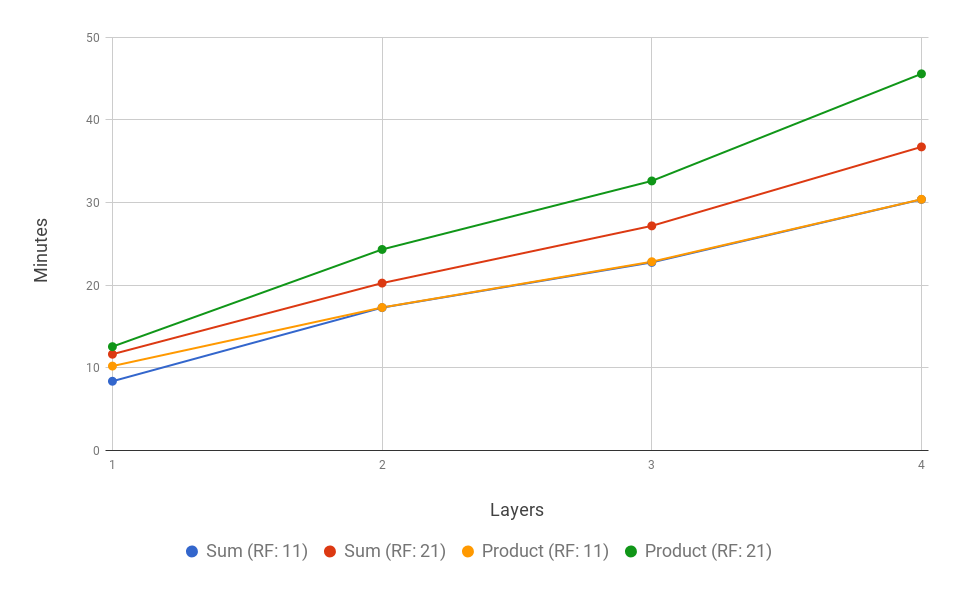
\includegraphics[width=0.8\textwidth]{training_times.png}
	\caption{Training time for pairwise graph convolution neural network, during testing. Times are shown for sum and product coupled convolutions, receptive fields of size 11 and 21, and 1-4 convolutional layers. Training time scales roughly linearly with the number of layers.
	\label{fig:train_times}}
\end{figure}

Graph convolutional networks were compared to PAIRpred, an existing state-of-the-art partner specific interface prediction algorithm based on an SVM with custom symmetric pairwise kernels, proposed by Minhas et al, (2014)~\cite{minhas2014}.
The original PAIRpred publication used different complexes, slightly different features, and a different experimental protocol, so it was run with.
Grid search with five-fold cross validation was used to select the optimal kernel and soft margin parameters.

The proposed graph convolution layers were also compared against diffusion convolutions, a spatial graph convolution proposed by Atwood and Towsley, (2016), designed to simulate a diffusion process across each vertex of an input graph~\cite{atwood2016}.
Diffusion convolutions generate a power series of a weighted adjacency matrix, where each matrix of the power series is the adjacency matrix raised to a unique power.
In their convolutions, all powers up to a certain limit (the maximum number of "hops").
This approach only supports a single weight on each edge, so in this case Gaussian normalized distances were used and relative angle was dropped. 
Manual model selection was used to identify the best values of the standard deviation parameter in the Gaussian normalization.

\section{Metrics}

Accuracy usually of interest in classification problem, but it's threshold dependent.
same goes for Precision, Recall, F measure, etc...
Thresholds can be found through model selection, but more straight forward to use threshold independent measures like the ROC curve, specifies true positive rate for an accepted false positive rate.
- AUC evaluates overall performance across all thresholds higher is better. 

Often biologists can learn a lot from just a few interacting pairs. 
We should have metrics which evaluate performance on just the top measures. 
One such measure is RFPP, lower is better.
%TODO: include this?: Another is RFPP PR1

AUC and RFPP can be computed for each complex individually, so we can measure the overall effectiveness of a method using the median value across all methods. 


\section{Results}

\subsection{Sum and Product Coupling Performance}

\begin{table}
	\begin{center}
		\begin{tabular}{lccccc}
			\toprule
			\multirow{2}{*}{Method} &
			Receptive Field & \multicolumn{4}{c}{Layers Before Merge} \\
			& Size & 1 & {2} & {3} & {4} \\
			\midrule
			No Convolution & N/A & \textbf{0.815} & 0.812 & 0.800 & 0.811  \\\cline{1-6}
			\multirow{2}{*}{GCN-SC} & 11 & 0.868 & 0.889 & 0.882 & 0.884 \\
			& 21 & 0.875 & \textbf{0.903} & 0.880 & 0.890 \\\cline{1-6}
			\multirow{2}{*}{GCN-PC} & 11 & 0.856 & 0.869 & 0.885 & 0.868 \\
			& 21 & 0.863 & 0.876 & 0.896 & \textbf{0.899} \\
			\bottomrule
		\end{tabular}
		\caption{Median area under the receiver operating characteristic curve (AUC) across all complexes in the test set for two variants of Graph Convolutional Networks (GCN), \textit{sum-coupled} (SC) and \textit{product-coupled} (PC). Results are shown for two different sizes of receptive field, 11 and 21, for different numbers of convolutional layers before the pairwise merge operation. Bold faced values indicate best performance for each method.}
		\label{tab:med_auc}
	\end{center}
\end{table}

\ref{tab:med_auc}
	- incorporating neighbor info helps b/c convolutions do better than no convolution
	- the larger receptive field tends to benefit as well. roughly the size of an average interface in the dataset (number? basir?).
	- Number of layers may be tends to help to a point, but then decreases (even for product coupling which is not shown).
		- best for no-convolution is 1 layer, suggesting that just is deeper better, but also that stacked convolutions help. this suggests a useful hierarchical representation is being learned. 
		- depth limit could be due to small amount of data.
		- vanishing gradient?
	- Sum coupling appears to do better, but AUC is only part of the story.
	
\begin{table}
	\begin{center}
		\begin{tabular}{lccccc}
			\toprule
			\multirow{2}{*}{Method} &
			Receptive Field & \multicolumn{4}{c}{Layers Before Merge} \\
			& Size & 1 & {2} & {3} & {4} \\
			\midrule
			No Convolution & N/A & \textbf{48} & 55 & 53 & 66 \\\cline{1-6}
			\multirow{2}{*}{GCN-SC} & 11 & 32 & 28 & 70 & 86 \\
			& 21 & \textbf{26} & 37 & 56 & 63 \\\cline{1-6}
			\multirow{2}{*}{GCN-PC} & 11 & 30 & 46 & 26 & 51 \\
			& 21 & 26 & \textbf{25} & 36 & 37 \\
			\bottomrule
		\end{tabular}
		\caption{Median rank of the first positive prediction (RFPP) across all complexes in the test set for two variants of Graph Convolutional Networks (GCN), \textit{sum-coupled} (SC) and \textit{product-coupled} (PC). Results are shown for two different sizes of receptive field, 11 and 21, for different numbers of convolutional layers before the pairwise merge operation. Bold faced values indicate best performance for each method (lower is better). For a given receptive field size and number of layers, product coupling performs better than sum coupling except for one case.}
		\label{tab:med_rfpp}
	\end{center}
\end{table}

\ref{tab:med_rfpp}
	- Here product coupling does same or better than sum coupling for all but one case.
	- product coupling detects more specific patterns since it associates each neighbor with its edge. So perhaps better able to detect the specific patterns indicitave of the most interface pairs.
	- remember, Algorithm is optimizing for overall loss, not RFPP.
	
\begin{figure}
	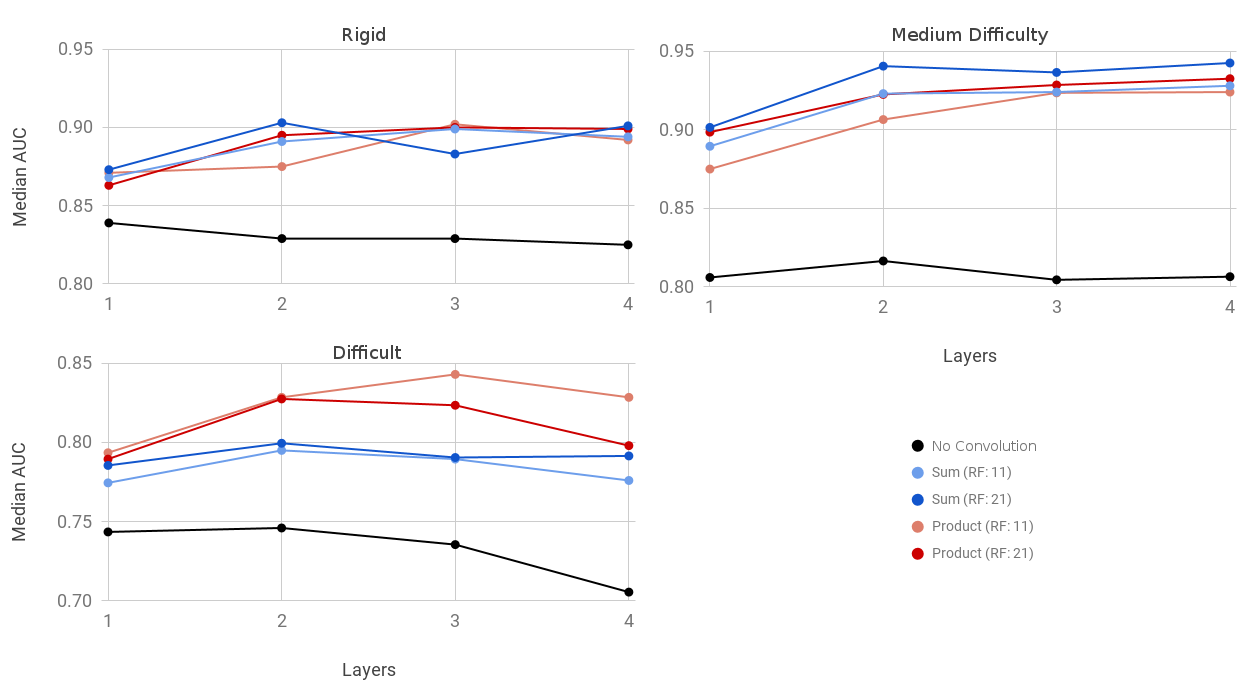
\includegraphics[width=\textwidth]{med_auc.png}
	\caption{Median area under the receiver operating characteristic curve (AUC) across all complexes in the test set, separated by complex class. Sum and product coupling are shown for two receptive field sizes each (11 and 21), as well as no convolution, for 1-4 pre-merge layers. Product coupling performs better for difficult complexes, but worse overall because ther are far more rigid and medium difficulty complexes.
		\label{fig:med_auc}}
\end{figure}
	
results more interesting when separate by difficulty:
33, 16, 6
\ref{fig:med_auc}
	- Sum and product coupling are closely matched for rigid and medium difficulty complexes, but product coupling clearly doing better on difficult complexes, especially for 2 and 3 layers. 
	- In overall performance, sum still wins out because there are only 6 hard complexes in the test set.
	
	
\begin{figure}
	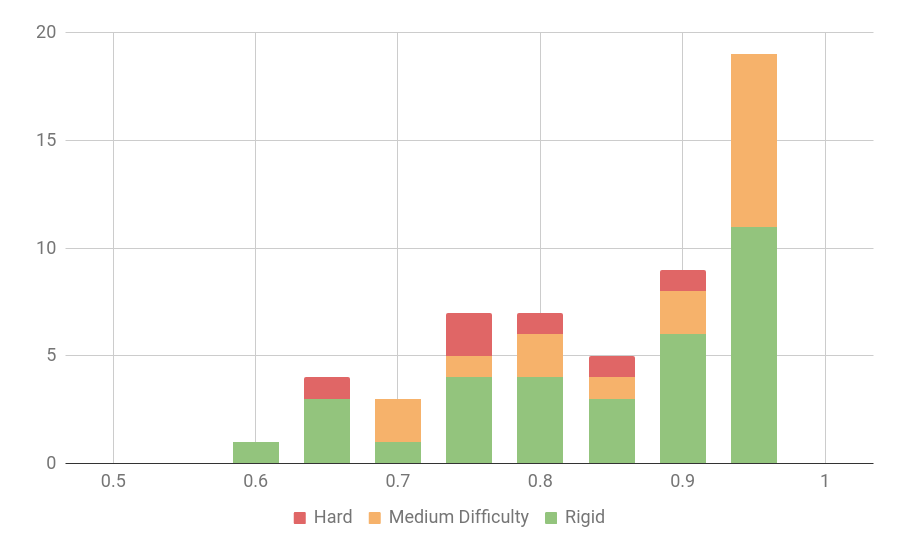
\includegraphics[width=0.8\textwidth]{sum_20_2_histo1.png}
	\caption{Histogram of area under the receiver operating characteristic curve (AUC) for proteins in the test set, colored by difficulty class. Scores are from sum coupled, graph convolution with two layers and receptive field size 21.}
	\label{fig:histo1}
\end{figure}

For another picture of performance across classes, look at histogram of AUC's
\ref{fig:histo1}
	- Note right skewness, which justifies use of median as a measure. 
	- Note that no clear divide between rigid, medium, and difficult residues. in fact, worst performing residue is rigid and one difficult gets at least a 0.90 AUC
	- instead, several easy medium appear to be almost "trivial", with scores above 0.95, whereas no difficult complexes exceed that threshold.
	
how about RFPP?
	
\begin{figure}
	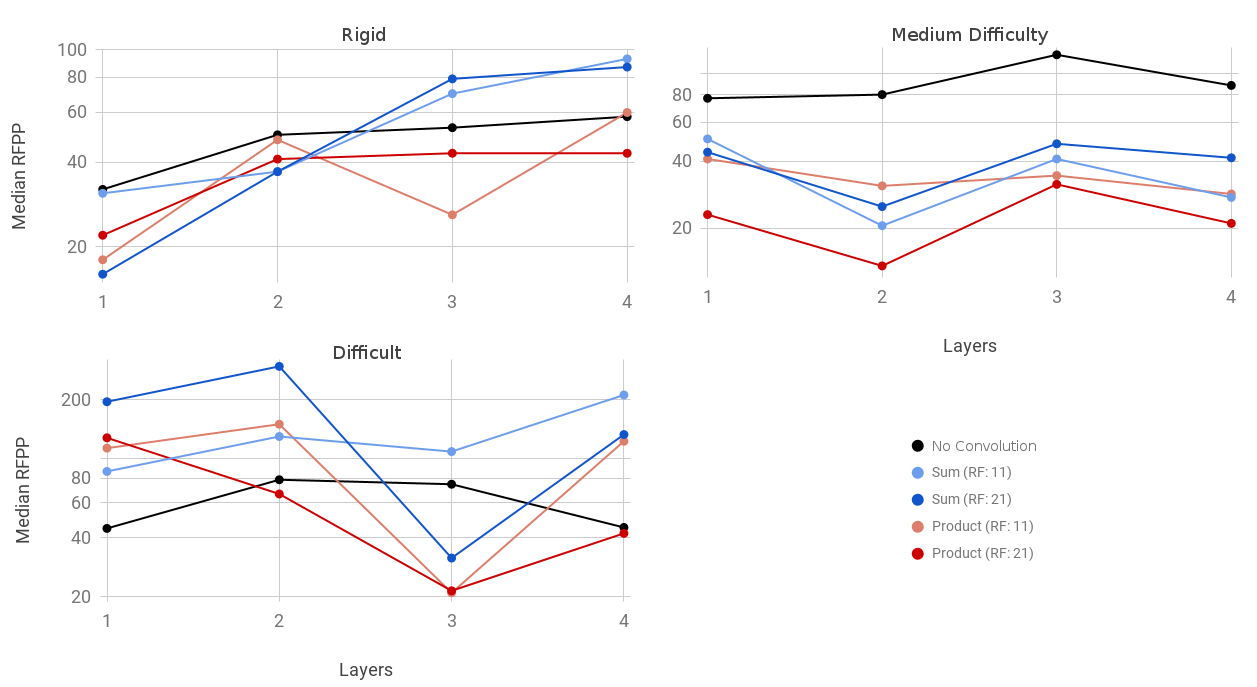
\includegraphics[width=\textwidth]{med_rfpp.png}
	\caption{Median rank of the first positive prediction (RFPP) across all complexes in the test set, separated by complex class. Vertical axes are log scaled. Sum and product coupling are shown for two receptive field sizes each (11 and 21), as well as no convolution, for 1-4 pre-merge layers. Lower RFPP is better. Best performance on rigid complexes is achieved with just one layer for all networks. As difficulty increases, so does the number of layers needed to achieve best results.
		\label{fig:med_rfpp}}
\end{figure}
	
\ref{fig:med_rfpp}
	- some heterogeneus behavior across methods, but some trends. 
	- For each class, there appears to be a favored number of layers, where depth increases with difficulty.



\subsection{Comparison to Prior Methods}



\begin{table}
	\begin{center}
		\begin{tabular}{l c c c c }
			\toprule
			\multirow{2}{*}{Method} & \multicolumn{4}{c}{Median AUC} \\
			& Overall & Rigid & Medium & Difficult \\
			\midrule
			2-hop DCNN ($\sigma=2$\AA{}) & 0.782 & 0.775 & 0.821 & 0.753 \\
			2-hop DCNN ($\sigma=4$\AA{}) & 0.801 & 0.820 & 0.817 & 0.681 \\
			\midrule
			5-hop DCNN ($\sigma=2$\AA{}) & 0.838 & 0.849 & 0.847 & 0.793 \\ 
			5-hop DCNN ($\sigma=4$\AA{}) & 0.819 & 0.832 & 0.867 & 0.740 \\ 
			\midrule
			PAIRpred      & 0.863        & & & \\
			\midrule
			GCN-SC (2 layers) & 0.903 & 0.903 & 0.941 & 0.800 \\ 
			\bottomrule
			\\
		\end{tabular}
		\caption{Comparison with existing classification methods. 
			PAIRpred is a state-of-the-art interface prediction method~\cite{minhas2014}, and DCNN is our implementation of the diffusion convolution method~\cite{atwood2016}.
			For DCNN, we used a single convolutional layer before merging, as more layers did not improve the performance (data not shown). DCNN performed better when the adjacency matrix consisted of a Gaussian function of distance, with a standard deviation of 2\AA{} and 4\AA{}, for 2 and 5 hops. Bold faced value indicates the best performance.}
		\label{tab:results_compare}
	\end{center}
	%\end{minipage}
\end{table}


\ref{tab:results_compare}
	- the proposed graph convolutions outperform both PAIRpred and diffusion convolutions, in every class.
	- pairpred 
	



diffusion based on graph connectivity, this is complete graph which might be noisy, explains why smaller stdev were better.

5 hop diffusion did better with smaller STDDEV since more information propagating through hops
2 hop diffusion did better with larger STDDEV since fewer hops limits information propagation.










%\chapter{Possible Future Work}
\label{chap:future}

The work in this thesis is pertinent to emerging methods in machine learning as well as current problems in structural bioinformatics.
As such, extensions of this work can be made in several distict veins, some focused on model formulation and training procedure, others on possible applications outside of interface prediction.
Several of these extensions are documented below, categorized as either extensions of method or extensions of application.

\section{Extensions of Method}

\subsection{Double Coupling and Ensemble Approaches}

As discussed in Chapter \ref{chap:experiments}, sum coupling outperforms product coupling on rigid and medium difficulty complexes, whereas product coupling is better for difficult complexes.
Therefore it would be reasonable to incorporate both sum and product coupling into a single convolution operation:

\begin{equation}
h_i(x | W^\textsc{c}, W^\textsc{n}, W^\textsc{e}, b) = \sigma \bigg( W^{\textsc{c}} x_i + \frac{1}{|\mathcal{N}_i|}\sum_{j \in \mathcal{N}_i} (W^{\textsc{n}} x_j) \odot (W^{\textsc{e}} A_{ij}) + W^{\textsc{n}} x_j + W^{\textsc{e}} A_{ij} + b \bigg),
\label{eq:double_coupling}
\end{equation}

\noindent
where here the same weight matrices are used in both the sum coupling and product coupling components to help prevent overfitting. 
Alternately, separate weight matrices could be used to increase the model's expressive power.

Recall that concerning the RFPP metric, the optimal network depth increased with complex difficulty, where more layers were needed for complexes of greater difficulty. 
This suggests that an ensemble model with multiple networks of varying depth could perform  better than each individual network.
Alternative ensemble approaches like \emph{boosting} or \emph{bagging} may also prove beneficial.
Boosting trains a sequence of "weak" models, with each added model being trained by giving more importance (loss weight) to examples misclassified by the existing set of models.
For interface prediction, this weighting can be performed on a per-complex basis, using RFPP or AUC as an indication of performance on each complex, or on a per-residue-pair basis, using the cross entropy loss of that specific training example.
The final prediction is a weighted average of the weak models' predictions, with the weights determined by the validation error of each respective model (with higher weight given to models with lower error).
Bagging creates multiple datasets by sampling with replacement from the original data set, and trains a different model on each sampled dataset.
This sampling can be performed at the complex level or the residue pair level.
Again, the final prediction is a weighted average of the weak models' predictions, weighted according to validation error.



\subsection{RFPP Optimization}

Predicting an entire interface is a more difficult task than predicting only a few interacting residues in that problem.
It could be that training a classifier in the former may hinder its performance in the latter.
An alternative approach would be to just focus on generating a few predictions of high quality (i.e. confidence), which means optimizing performance on just the top positive predictions.
The existing model uses a loss function which incorporates every training example, not just the top positive prediction, hence the model is optimized for all examples.
This implies treating RFPP as the primary metric and optimizing it directly.
An alternate loss function which includes the loss from only the highest scoring positive example could be used.
Hence when the loss is minimized, the performance of the highest performing positive example will be maximized.
Here a sum over all examples has been replaced by a max function, which is not differentiable, but differentiable variants of the loss function could be constructed to enable gradient descent based learning.
This method is currently being investigated by another student in Professor Ben-Hur's research group.

\subsection{Additional Data Sources}

The success of deep learning methods has been attributed to large volumes of data and deep architectures~\cite{krizhevsky2012}.
For interface prediction, despite the large volume of recorded protein structures, precious few complexes have been labeled in bound and unbound forms for use in model training and testing. 
This dependence on small curated subsets of the available proteins has potentially limited the full leveraging of deep learning methods, however some opportunities exist for enlarging the training and testing data.

The Docking Benchmark Dataset was conceived as a method to evaluate docking methods, and correspondingly was carefully constructed to be non-redundant with respect to SCOP families, in order to give a fair evaluation.
However for training purposes, it may be useful to include redundant proteins simply to provide the model with more training data. 
The Critical Assessment of PRediction of Interactions (CAPRI) is an annual competition aimed at evaluating protein-protein docking methods~\cite{janin2003}, and could also be used to help train or evaluate partner-specific protein interface prediction methods. 

\subsection{Unsupervised Pretraining}

Another approach to the problem of limited labeled complexes is to utilize the vast quantity (>125,000) of recorded protein structures via unsupervised pre-training.
Hinton and Salakhutdinov (2006)~\cite{hinton2006b} proposed a greedy layer-wise training algorithm for a particular form of neural network called an \emph{autoencoder}.
Generally speaking, an autoencoder is simply a network trained to reproduce the input at the output under certain constraints~\cite{goodfellow2016}.
These constraints, such as undercompleteness, regularization, and sparsity, prevent the network from simply learning an identity mapping of the input, and instead promote the learning of a compressed representation of the input (i.e. an "encoding").
The portion of the network which compresses the input is called the encoder, while the portion which reconstructs the input from the encoding is called the decoder.
The encoding half of the autoencoder can be used independently of the decoding half to create representations of the input that are often useful in supervised tasks like classification~\cite{hinton2006b, bengio2007}.

Masci et al (2011)~\cite{masci2011} proposed convolutional autoencoders (CAEs) which perform convolution to encode an image and \emph{deconvolution} to decode the image.
There is also a corresponding \emph{unpooling} operation which upsamples images which were pooled during the encoding step.
Deconvolution is simply a convolution operation performed on the result of an encoding convolution, with weights being tied between convolution and deconvolution layers.
For $k$ filters of size $m \times m$ and $c$ channels, the corresponding deconvolution would consist of $c$ filters of size $m \times m$ and $k$ channels, where the weights have been reflected in both spatial dimensions (e.g. the weights for the lower left pixel of the receptive field are now applied to the upper right pixel).
The spatial reflection allows a particular weight to carry a specific meaning, namely it characterizes the relationship between a particular pixel in an image and a pixel in its encoding.
To illustrate this, Figure \ref{fig:deconv} shows a deconvolution for a single filter and single channel.
CAEs are trained in the same greedy, layerwise fashion as conventional autoencoders.

\begin{figure}
	\includegraphics[width=0.8\textwidth]{conv_ae.png}
	\caption{Application of convolution, then deconvolution on a single channel input image. The relationship between the purple pixel in the input/reconstruction and the red pixel in the encoding is captured by the appropriate weight in the filters (lower left for convolution and upper right for deconvolution). By reflecting the convolution filter horizontally and vertically for use in deconvolution, the same weight ($W_{31}$) is used for this relationship during both encoding and decoding.
		\label{fig:deconv}}
\end{figure}


The concept of deconvolution can be applied to graph convolutions as well.
Note that when reflecting image convolution filters, the center weight remains in the same position.
In the same way, graph deconvolutions retain the same weights for the central vertex. 
Furthermore, since all neighbors use the same weights, there is no spatial reflection necessary.
Deconvolution simply consists of transposing the center and neighbor weight matrices so that channels become filters and filters become channels.
For sum coupling, deconvolution becomes:

\begin{equation}
\hat{x_i}(h_i | W^\textsc{c}, W^\textsc{n}, W^{\textsc{e}*}, b^*) = \sigma \bigg( (W^{\textsc{c}})' h_i + \frac{1}{|\mathcal{N}_i|}\sum_{j \in \mathcal{N}_i} \big[ (W^{\textsc{n}})' h_j + W^{\textsc{e}*} A_{ij} \big] + b^* \bigg),
\label{eq:sum_deconv}
\end{equation}

\noindent
where $\hat{x}$ denotes the reconstruction of $x$ after deconvolving, $h_i$ is the convolved representation at vertex $i$, $(W^\textsc{c})'$ is the transpose of $W^\textsc{c}$, likewise for $(W^\textsc{n})'$ and $W^\textsc{n}$, and both $W^{\textsc{e}*}$ and $b^*$ are weight matrices with unshared weights. 
Note that graph convolutions generate representations on vertices of the graph, not the edges, so the non-encoded edge information ($A_{ij}$) must be used when deconvolving, and the weight matrix $W^{\textsc{e}*}$ cannot be tied to the encoding matrix $W^{\textsc{e}}$.

Alternately, edge representations could be created in a separate convolution operation, where an edge's receptive field is simply the incident vertices:

\begin{equation}
h_{ij}(A_{ij} |W^{\textsc{ee}}, W^{\textsc{ev}}, b_e) = \sigma\bigg( W^{\textsc{ee}} A_{ij} + \frac{1}{2}\big(
W^{\textsc{ev}} x_i + W^{\textsc{ev}} x_j \big) + b_\textsc{e} \bigg),
\label{eq:edge_conv}
\end{equation}

\noindent
where $h_{ij}$ is the representation of edge $(i, j)$ , $W^{\textsc{ee}}$ is the weight matrix associated with the edge, and $W^{\textsc{ev}}$ is the weight matrix associated with the incident vertices.
In this case, vertex deconvolution can use the encoded edge representations and associated weights.
Equation (\ref{eq:sum_deconv}) then becomes:

\begin{equation}
\hat{x_i}(h_i | W^\textsc{c}, W^\textsc{n}, W^\textsc{v}, b) = \sigma \bigg( (W^{\textsc{c}})' h_i + \frac{1}{|\mathcal{N}_i|}\sum_{j \in \mathcal{N}_i} \big[ (W^{\textsc{n}})' h_j + (W^{\textsc{ev}}) h_{ij} \big] + b^* \bigg),
\label{eq:sum_deconv2}
\end{equation}

\noindent
where $(W^{\textsc{V}})'$ is the transpose of $W^{\textsc{V}}$.
Edges can also be deconvolved using the edge and vertex representations:

\begin{equation}
\hat{A_{ij}}(h_{ij} | W^{\textsc{ee}}, W^{\textsc{e}}, b) = \sigma \bigg( (W^{\textsc{ee}})' h_{ij} + \frac{1}{2}\big[
(W^{\textsc{e}})' h_i + (W^{\textsc{e}})' h_j \big] + b^{*}_\textsc{e} \bigg).
\label{eq:edge_deconv}
\end{equation}

\noindent
This added weight sharing and symmetry between convolution and deconvolution operations may allow training of deeper networks which recognize more sophisticated structures.



\subsection{Simplicial Complex Convolution}

Graphs are only one way to model structural relationships between entities.
A simplicial complex is a generalization of a graph in which higher order simplices (triangles, tetrahedra, etc), in addition to edges, describe relationships between groups of vertices. 
For example, just as an edge indicates a relationship between two vertices, a triangle (or 2-simplex) indicates the relationship between three vertices.
For example, both the \v{C}ech and Vietoris-Rips definitions can be used to construct a simplicial complex from a set of points in an underlying metric space:

\begin{definition}
	Given a point set $X$ in some metric space and a number $\epsilon>0$, the \v{C}ech complex $C^{\textsc{\v{C}}}_\epsilon$ is the simplicial complex whose simplices are formed as follows. For each subset $S \subset X$ of points, form an ($\epsilon/2$)-ball around each point in $S$, and include $S$ as a simplex (of dimension $|S|$) if there is a common point contained in all of the balls in $S$.
\end{definition}

\begin{definition}
	Given a point set $X$ in some metric space and a number $\epsilon>0$, the Vietoris-Rips complex $C^{\textsc{VR}}_\epsilon$ is the simplicial complex whose simplices are formed as follows. For each subset $S \subset X$ of points, form an ($\epsilon/2$)-ball around each point in $S$, and include $S$ as a simplex (of dimension $|S|$) if for each pair of balls in $S$ there is a common point contained in both balls.
\end{definition}

In both definitions, simplices are included in the simplicial complex based on some notion of proximity.
This means simplicial complexes are naturally equipped to identify clusters of vertices within a neighborhood, something which can be useful for interface prediction, where local regions of residues may constitute portions of an interface.
Though the number of possible convolution operations on simplicial complexes are many, one example is provided here for the purpose of discussion. 
In this formulation, rather than sum the signal from all neighbors in the receptive field, each simplex $S_k, k \in \{1, 2,... K\}$ (not counting vertices and edges, which are the lowest order simplexes) in the neighborhood is summed individually and the maximum simplex signal is added to the central signal:

\begin{equation}
\begin{split}
h_i(x |  & W^{\textsc{c}}, W^{\textsc{n}}, W^{\textsc{e1}}, W^{\textsc{e2}}, b) = \\ 
&\sigma \bigg( W^{\textsc{c}} x_i + \max_{k} \Big[ \frac{1}{|S_k|}  \sum_{j \in \mathcal{S}_k} ( W^{\textsc{n}} x_j + W^{\textsc{e1}} A_{ij} ) + \frac{1}{|S_k|^{2}}\sum_{j, l \in \mathcal{S}_k} (W^{\textsc{e2}} A_{jl}) \Big] + b \bigg).
\end{split}
\label{eq:simplicial_complex_conv}
\end{equation}

\noindent
This formulation also includes \emph{secondary} edges ($A_{jl}$), those between different neighbors in the same simplex.
It is possible that neighbors and edges occur in more than one simplex in the neighborhood, but that doesn't pose a problem because of the normalization and max function.
The use of simplicial complexes in defining convolution operations is currently being investigated by a student in Professor Ben-Hur's research group.


\section{Extensions of Application}

Interface prediction is not the only active area of protein research, and so the modeling of proteins as graphs and use of graph convolution could potentially be used for other protein problems as well.
A common characteristic of docking methods is that they create a high number of putative 3D bound structures~\cite{janin2013}.
Graph convolutional neural networks could also be used to evaluate putative docking solutions and rank them in order of likelihood.
For example, the interface derived from a docking solution could be compared to the interface predicted by a trained pairwise graph convolutional neural network and ranked according to similarity with the network prediction.
Similarly, much research has been performed in protein modeling, which seeks to predict a protein's secondary and tertiary structures from sequence alone~\cite{schwede2013}.
Though graph convolutions cannot be used to create protein folds \emph{de novo}, they can be used to evaluate a set of putative folds and likewise rank them.
In both of these applications, regression is being performed not at the individual vertex level, but at the graph level.
These could take advantage of a global pooling method like taking the maximum or average across all vertices, or developing a \emph{fingerprint} similar to work by Duvenaud \& Maclaurin, et al.~\cite{duvenaud2015}.

Any application involving structured data that do not fit naturally into a grid is a potential candidate for graph convolutional approaches.
Aside from proteins, other biological and chemical data often meet this criterion.
In particular, Quantitative Structure-Activity Relationship (QSAR) and Quantitative Structure-Property Relationship (QSPR) both attempt to predict chemical behavior and properties of proposed chemical structures in order to identify structures with certain desired properties. 
Identified structures become candidates for laboratory synthesis and experimentation, a much more laborious and time consuming process. 
This is the focus of the Fingerprint convolution from Duvenaud \& Maclaurin et al.~\cite{duvenaud2015}.
Studies in QSAR and QSPR have long been considered "unquestionably of great importance in modern chemistry and biochemistry"~\cite{karelson1996}.
Like proteins, chemical structures can be modeled as a graph and used to train graph convolutional networks to predict the properties of interest.
This is made possible by the vast and growing databases of chemical structures and their corresponding structures~\cite{olah2008, judson2008}.

Beyond the biochemical realm, graph structured data abound.
Knowledge bases are collections of structured data in the form of triples indicating \emph{(subject, predicate, object)}, where \emph{subject} and \emph{object} are named entities and \emph{predicate} indicates the relationship between them, and pairs indicating \emph{(subject, attribute)}, where \emph{attribute} is a type or property label for \emph{subject}.
These data can easily be thought of graphs, where entities are vertices each type of predicate is one of many different types of edge features, and each attribute is one of many different types of vertex features.
Knowledge bases emerge in online information repositories such as YAGO~\cite{mahdisoltani2014}, DBPedia~\cite{auer2007}, and Wikidata~\cite{vrandevcic2014}, and are used in the Google search engine \cite{singhal2012}.
Due to their large size, knowledge graphs are often under-annotated, where vertex relationships and properties are missing. 
A graph convolutional neural network can be used to predict properties or relationships on graphs, essentially performing automatic inference on the graph.








\backmatter % starts unnumbered supplementary material
%%%%%%%%%%%%%%%%%%%%%%%%%%%%%%%%%%%%%%%%%%%%%%%%%%%%%%%%%%%%%%%%

% Bibliography
%%%%%%%%%%%%%%%%%%%%%%%%%%%%%%%%%%%%%%%%%%%%%%%%%%%%%%%%%%%%%%%%

% unsorted BibTeX style
% check here for more:  https://www.sharelatex.com/learn/Bibtex_bibliography_styles
\bibliographystyle{unsrt}
\bibliography{biblio} % change readme to the name of your .tex file

\appendix % starts the appendices
%%%%%%%%%%%%%%%%%%%%%%%%%%%%%%%%%%%%%%%%%%%%%%%%%%%%%%%%%%%%%%%%

\chapter{Features}
\label{appendix:features}

The raw data associated with protein structures are found in PDB files, which contain the protein sequence of amino acids and the atomic coordinates of each atom in each amino acid.
When performing interface prediction, a number of derived features have been found useful, which are either calculated directly from the PDB data, or from other sources such as sequence databases.
Here, the term \emph{features} describes a vector of values associated with either a vertex or edge in a graph, with vertices corresponding to amino acid residues, and edges the relationships between two residues.
The term \emph{feature} then is just a single element of the vector.
Some methods described below generate more than one feature, hence they are grouped into appropriate \emph{categories}.
This appendix describes each feature category in detail, including the number of features generated, external tools, and a description of the feature.
In addition to the tools specified for each feature category, extensive use was made of Biopython~\cite{cock2009} to parse PDB files into convenient data structures. 

\section{Vertex Features}

\subsection{Windowed Position Specific Scoring Matrix (PSSM)}
\noindent
\emph{Number of features}: 20

\noindent
\emph{External tools}: PSI-BLAST~\cite{altschul1997}

\noindent
\emph{Description}:
The PSSM is a set of features constructed from protein sequence alone, without any structural information.
It captures the relative abundance of each type of amino acid in proteins which share a similar sequence in a window around the amino acid of interest.
Proteins with similar sequences to the search window are identified through PSI-BLAST, a position specific, iterative version of BLAST, the Basic Local Alignment and Search Tool~\cite{altschul1990}.
The similar sequences are then used to generate a summary in a window around the residue of interest.
For each window position and each residue type, a score is computed by comparing the observed counts of that residue type in that window position to the expected count generated by a null model.
The score is then $\log(Q_i/P_i)$ where $Q_i$ is the fraction of sequences with that residue type in that position, and $P_i$ is the expected fraction based on data-dependent pseudocounts (more detail can be found in Altschul, et al.~\cite{altschul1990}.
For this thesis, only the scores at the residue of interest were considered (a window size of one), so there are 20 features, one for each amino acid type. 

\subsection{Relative Accessible Surface Area (rASA)}
\noindent
\emph{Number of features}: 1

\noindent
\emph{External tools}: STRIDE~\cite{heinig2004}

\noindent
\emph{Description}:
Relative Accessible Surface Area, or \emph{Solvent Accessible Area}, reflects the fraction of a residue that is exposed to a potential solvent.
This is computed by sliding a spherical probe of radius of 1.4\AA{} (approximating the radius of a water molecule~\cite{eisenhaber1995}) over the van der Waals surface of the protein near the residue of interest.
The Area generated by the center of the probe as it is in contact with the residue is taken to be the accessible surface area.
This is divided by the maximum possible accessible surface area to achieve a relative measure.


\subsection{Residue Depth}
\noindent
\emph{Number of features}: 2

\noindent
\emph{External tools}: MSMS~\cite{sanner1996}

\noindent
\emph{Description}:
Residue Depth is the minimum distance from the residue to the surface of the protein, as calculated by MSMS.
The distance is calculated is two ways: by taking the average distance of all non-hydrogen atoms in the residue to the surface, and by taking the distance of the $\alpha$-carbon to the surface.


\subsection{Protrusion Index}
\noindent
\emph{Number of features}: 6

\noindent
\emph{External tools}: PSAIA~\cite{mihel2008}

\noindent
\emph{Description}:
The protrusion index indicates the degree to which a sphere (radius 10\AA{}) centered at a non-hydrogen atom is not filled with other atoms.
$V_{int}$ is the volume occupied by atoms, which is calculated as the number of atoms times the mean atomic volume found in proteins.
$V_{ext}$ is the difference between the total sphere volume and $V_{int}$. 
The protrusion index is defined as $V_{ext}/V_{int}$.
This value is calculated for each non-hydrogen atom in the residue, then the following summary statistics are taken:
\begin{itemize}
	\item \emph{Total mean}: The average over all non-hydrogen atoms in the residue
	\item \emph{Total standard deviation}: The standard deviation over all non-hydrogen atoms in the residue
	\item \emph{Side chain mean}: The average over just non-hydrogen atoms in the residue side chain
	\item \emph{Side chain standard deviation}: The standard deviation over just non-hydrogen atoms in the residue side chain
	\item \emph{maximum}: The maximum over all non-hydrogen atoms
	\item \emph{minimum}: The minimum over all non-hydrogen atoms
\end{itemize}
All of these features are normalized to values between 0 and 1 on a per-protein basis.


\subsection{Hydrophobicity}
\noindent
\emph{Number of features}: 1

\noindent
\emph{External tools}: PSAIA~\cite{mihel2008}

\noindent
\emph{Description}:
Hydrophobicity indicates the tendency for an amino acid to avoid water.
PSAIA calculates this value base on the scale defined by Kyte \& Doolittle~\cite{kyte1982}.
Hydrophobicity values were normalized between 0 and 1 on a per-protein basis.


\subsection{Half Sphere Amino Acid Composition}
\noindent
\emph{Number of features}: 40

\noindent
\emph{External tools}:  None

\noindent
\emph{Description}:
These features capture the residue composition in a neighborhood of the residue of interest.
The neighborhood is defined as all residues with at least one atom closer than 8\AA{} to at least one atom in the residue of interest.
An array of counts is created which stores the number of each type of residue in the neighborhood, which is then divided by the total count of all types.
This array is calculated for two regions, separated by the null space of the vector that is the average of the unit vectors from the $\alpha$-carbon to the side chain atoms.


\section{Edge Features}

\subsection{Average Atomic Distance}
\noindent
\emph{Number of features}: 1

\noindent
\emph{External tools}: None

\noindent
\emph{Description}:
This feature is computed by taking the average of the distance between any two atoms of the two residues of interest.
The raw distance is then passed through a Gaussian function: 

\begin{equation}
f(x) = e^{-x^2 / \sigma^2},
\end{equation}

\noindent
where $\sigma$ is chosen by model selection, so that this feature has a higher value for residues that are closer together.


\subsection{$\text{CC}_{\alpha} \text{O}$ Angle}
\noindent
\emph{Number of features}: 1

\noindent
\emph{External tools}: None

\noindent
\emph{Description}:
This feature captures the relative orientation of two residues as defined by the normals to their adjacent peptide planes.
Let $X_{C_{\alpha}}$, $X_{C}$, and $X_{O}$ be the positions vectors of the $\alpha$-carbon, carboxyl-group carbon, and carboxyl-group oxygen respectively.
The normal is then defined as:
\begin{equation}
\hat{N} = \frac{(X_{O} - X_{C}) \times  (X_{C_\alpha} - X_{C})}{||(X_{O} - X_{C}) \times  (X_{C_\alpha} - X_{C})||}, 
\end{equation}

\noindent
where $\times$ denotes the cross product, and $ || \cdot || $ the $\textsc{L}^2$ norm.
The angle between residues $i$ and $j$ is then:
\begin{equation}
\text{C C}_{\alpha} \text{O} = \text{cos}^{-1}\bigg(\frac{\hat{N_i} \cdot \hat{N_j}}{|| \hat{N_i} ||~|| \hat{N_j} || } \bigg)
\end{equation}

\noindent
Finally, the angle is normalized to be between 0 and 1 by dividing by $2 \pi$. 



\section{Missing Data}
In Section \ref{sect:missing_data} it was noted that 13 residues were not provided with an $\alpha$-carbon in the corresponding PDB file. 
These residues were determined to be partial records at the end of a protein chain, where only a single atom was listed.
This made calculation of Half Sphere Amino Acid Composition, Residue Depth, and $\text{CC}_{\alpha} \text{O}$ Angle impossible.
Upon inspection, these partial records were deemed to be legitimate residues and so were retained, with the missing features imputed according to the procedure described in Chapter \ref{chap:experiments}.

\chapter{Tools}
\label{appendix:tools}


%%%%%%%%%%%%%%%%%%%%%%%%%%%%%%%%%%%%%%%%%%%%%%%%%%%%%%%%%%%%%%%%


%%%%%%%%%%%%%%%%%%%%%%%%%%%%%%%%%%%%%%%%%%%%%%%%%%%%%%%%%%%%%%%%
\end{document}
